\documentclass[twoside,11pt]{article}
\usepackage{jair,theapa,rawfonts}

\usepackage{amsmath}
\usepackage[algo2e,ruled,vlined,linesnumbered]{algorithm2e}
\SetKw{Continue}{continue}

\usepackage{amsthm,amssymb}
\usepackage{graphicx}
\usepackage{latexsym}
\usepackage{colortbl}
\usepackage[caption=false]{subfig}
\usepackage[bottom]{footmisc}
\usepackage{url}

\usepackage{booktabs,multirow}
\usepackage{xspace}

\usepackage[smaller]{acronym}
\acrodef{SPP}{Shortest Path Problem}
\acrodef{kUCS}{$k$ Uniform Cost Search}

\usepackage{wasysym}
\usepackage{pifont}% http://ctan.org/pkg/pifont
\newcommand{\cmark}{\textcolor{green}{\ding{51}}}
\newcommand{\xmark}{\textcolor{red}{\ding{55}}}

\usepackage{mathtools}
\DeclarePairedDelimiter{\ceil}{\lceil}{\rceil}
\DeclarePairedDelimiter{\floor}{\lfloor}{\rfloor}

\usepackage{tikz}
\usetikzlibrary{arrows,shapes,positioning,mindmap}

\newtheorem{theorem}{Theorem}
\newtheorem{definition}[theorem]{Definition}
\newtheorem{lemma}[theorem]{Lemma}
\newtheorem{corollary}[theorem]{Corollary}
\newtheorem{proposition}[theorem]{Proposition}
\newtheorem{observation}[theorem]{Observation}

%\newcommand{\kgs}{$k$-goal problem}
\newcommand{\kgs}{$k$GP\xspace}
\newcommand{\kgbfs}{$k$-goal best-first search\xspace}

\newcommand{\astar}{A$^*$\xspace}
\newcommand{\kastar}{kA$^*$\xspace}
\newcommand{\kastarvar}[1]{\textup{kA}$^*_{#1}$\xspace}
\newcommand{\kastarmin}{\kastarvar{\min}}
\newcommand{\kastarmax}{\kastarvar{\max}}
\newcommand{\kastarphi}{\textup{kA}$^*_{\Phi}$\xspace}
\newcommand{\kxastar}{k$\times$A$^*$\xspace}
\newcommand{\astari}[1]{A$^*_{#1}$\xspace}
%\newcommand{\newcode}[1]{{\color{blue}[+] #1}}
\newcommand{\newcode}[1]{#1}

\newcommand{\minf}{$F_{min}(n)$\xspace}
\newcommand{\maxf}{$F_{max}(n)$\xspace}
\newcommand{\tuple}[1]{\ensuremath{\left \langle #1 \right \rangle }}
\newcommand{\open}{\textsc{Open}\xspace}
\newcommand{\closed}{\textsc{Closed}\xspace}
\newcommand{\activeg}{\mathcal{A}}
\newcommand{\respog}{\mathcal{R}}
\newcommand{\extendedg}{\mathcal{E}}
\newcommand{\axiomadm}{adm-compat\xspace}
\newcommand{\axiomcons}{cons-compat\xspace}

\newcommand{\vect}[1]{\mathbf{#1}}
\newcommand{\nonnegreals}{\mathbb{R}_{\geq 0}}

\DeclareMathOperator*{\argmin}{arg\,min}
\DeclareMathOperator*{\argmax}{arg\,max}
%\newcommand{\argmin}{\operatornamewithlimits{argmin}}
%\newcommand{\argmax}{\operatornamewithlimits{argmax}}


\tikzset{style={>=stealth'}}
\tikzset{solution/.style={->,>=stealth',purple,dashed,bend left}}
\tikzset{source/.style={circle,    fill=white,draw=blue, text=blue, minimum size=7mm,inner sep=0mm}}
\tikzset{target/.style={circle,    fill=white,draw=red,  text=red,  minimum size=6mm,inner sep=0mm}}
\tikzset{target1/.style={rectangle,fill=white,draw=red,  text=red,  minimum size=6mm,inner sep=0mm}}
\tikzset{target2/.style={diamond,  fill=white,draw=red,  text=red,  minimum size=8mm,inner sep=0mm}}
\tikzset{targetk/.style={star,     fill=white,draw=red,  text=red,  minimum size=8mm,inner sep=0mm}}
\tikzset{other/.style={circle,     fill=white,draw=black,text=black,minimum size=7mm,inner sep=0mm}}
\tikzset{edgeweight/.style={align=left,font=\footnotesize,minimum size=6mm}}
\tikzset{infobox/.style={align=left,font=\footnotesize,minimum size=6mm}}



\newcommand{\roni}[1]{\textbf{[RS:#1]}}
\newcommand{\abda}[1]{\textbf{[AS:#1]}}
%\newenvironment{proof}{\noindent{\bf Proof:~~}}{\qed}


\jairheading{?}{???}{?-??}{?/??}{?/??}
\ShortHeadings{Shortest Path for K Goals}
{Stern, Goldenberg, Saffidine, \& Felner}
\firstpageno{1}

\begin{document}

\title{Heuristic Search for Finding Shortest Paths for K Goals}

\author{\name Roni Stern \email roni.stern@gmail.com \\
       \addr Ben Gurion University of the Negev, \\ Be'er Sheva, Israel
	   \AND
	   \name Meir Goldenberg \email mgoldenbe@gmail.com \\
       \addr The Jerusalem College of Technology, \\ Jerusalem, Israel
       \AND
       \name Abdallah Saffidine \email abdallah.saffidine@gmail.com \\
       \addr The Australian National University, \\ Canberra, Australia
       \AND
       \name Ariel Felner \email felner@bgu.ac.il \\
       \addr Ben Gurion University of the Negev, \\ Be'er Sheva, Israel}
	      

% For research notes, remove the comment character in the line below.
% \researchnote

\maketitle


\begin{abstract}
  In this paper we study the $k$ goal search problem (\kgs), which is the problem of solving $k$ shortest path problems that share the same start state.
  Two fundamental heuristic search approaches are analyzed: searching for the $k$ goals one at a time, or searching for all $k$ goals as a a single compound goal in a single pass.
  The former approach, denoted \kxastar, is simpler to implement, but can be computationally inefficient.
  We proposed several ways to implement the latter approach, denoted \kastar, and analyze their theoretical properties.
  Then, we analytically compare the runtime and memory requirements of \kxastar and \kastar, identifying when each approach should be used.
  Finally, we compare these approaches experimentally on two representative domains, providing empirical support for our theoretical analysis.
%    Finally, we compare these approaches experimentally on two different domains --- grid pathfinding and $n$-pancake puzzle --- providing empirical support for our theoretical analysis.
\end{abstract}


\section{Introduction and Motivation}

% SPP is classical, important and super general

The \ac{SPP} in a graph is a fundamental problem in Computer
Science, with many applications in Artificial Intelligence and Operations Research.
The input to an SPP problem is a graph and two vertices --- a \emph{start} vertex and a \emph{goal} vertex --- and the task is to find the lowest-cost path in the graph from start to goal.
Classical algorithms such as Dijkstra's algorithm~\cite{DIJ59} and \astar~\cite{hartNR68Astar} have been proposed for solving SPP.
SPP algorithms have been applied to various types of graphs.
In some cases, the graph is given explicitly, e.g., representing roadmaps, grids and game maps~\cite{sturtevant2012benchmarks}.
In other cases, the graph is defined implicitly by an initial vertex and a set of transition functions, e.g., representing a space of possible robot configurations, puzzle permutations, or STRIPS-like states in a domain-independent planning problem.
%[[AF: do we want references?]]\roni{Sure, any ideas what to add here?}


% We talk about k SPP

This paper addresses a generalization of SPP, where the task is to solve $k$ SPP problems, such that all the problems share the same start vertex.
That is, we have a single start vertex and $k$ goal vertices, and the task is to find $k$ shortest paths, where each path is a shortest path from the start to a different goal. 
We denote this problem as the \emph{$k$-goal} shortest path problem, or in short \kgs. %[[AF: you generalize SPP then maybe call it KG-SPP. Alternatively, do not use SPP, or say KGSPP and in short KGP]]


% k-goal is not TSP

\kgs is related to but is fundamentally different from previously studied problems such as the traveling salesman problem (TSP) and incremental search~\cite{koenig2004lifelong}.
In TSP, the task is to find a single path that passes through a set of vertices.
By contrast, in \kgs we aim for $k$ paths, one per goal.
In incremental search we have a single goal and the underlying graph changes.
By contrast, in \kgs the underlying graph does not change, and we are given the $k$ goals upfront. % and the task is to find paths for all these goals.
[[AF: different: Yes. Related to?? Explain why?]

% Motivation 1. Decision making
\kgs has many applications. Assume an interactive tour-planning application and a family planning a vacation with it.
Say that the family wishes to visit an amusement park and our tour-planning application finds $k$ amusement parks in the area.
Modeling the exact preferences of each family member and reconciling them is difficult if not impossible.
Thus, our application will output these $k$ parks.
Since the cost of getting to the amusement park is an important factor to consider when deciding which park to choose, our tour-planning application needs also to output the cost of getting to each of these $k$ parks.
This is exactly a \kgs problem, where the start vertex is the family's home and the goals are the $k$ different amusement parks. %[[AF: indeed this is my family]]

This tour-planning example represents a more general scenario that occurs when developing an intelligent personal assistant with a planning component~\cite{myers2007intelligent,chalupsky2001electric}.
The planning component may be decoupled from the agent's high-level decision making component, e.g., when following a Believe-Desire-Intention (BDI) architecture~\cite{bratman1999intention,georgeff1998belief}.
In such cases there may be multiple ($k$) alternative goals an agent may wish to achieve.
The cost of achieving them is an important input to the agent's decision making module, to decide which goal to aim for.
Computing the cost of achieving each of these $k$ goals is exactly an instance of \kgs{}. %[[KGP problem, the word problem appear twice]

%[[AF: Do we want to add Vitali's domain as another example, and add him too as a co-author?]][[Roni: No. It did not convince cyber people]

% Robotics
Efficient solutions to the \kgs problem can also be helpful in robotics.
For example, a path planning engine for multiple drones flying from a a central dispatcher location to $k$ target locations will need to solve the \kgs\ problem.
Another robotic application is when using the Incremental Roadmap Spanner technique~\cite{marble2013asymptotically}, which is a motion planning technique that requires searching for a shortest path to a limited number of nearby locations to speedup solving future pathfinding problems.
In fact, preliminary work on using heuristic search to solve \kgs was done exactly for this problem~\cite{DobsonB14}.
%[[AF: state exactly which of our versions they used. For example, say: they used a variant of the KMIN algorithm presented below.]]\roni{We can't say that here because we did not introduce our algorithms.  But it is good to say that later TODO}


A trivial algorithm for solving \kgs is to run a SPP solver $k$ times, one for each goal.
We refer to this algorithm as \kxastar.
\kxastar potentially explores parts of the search space multiple times, introducing redundant overlaps and missing opportunities for sharing information between the $k$ searches. 

The first contribution of this work is in exploring a range of alternative ways to share information between the different searches. We then focus on a framework of \kgs{} algorithms in which the $k$ goals are searched together in a single pass. 
We refer to this algorithmic search framework as \kastar. 

A challenge in \kastar is how to choose which node to expand next. 
In \astar{}, this is done by considering for every candidate node its distance to the starting point and a heuristic estimate of its distance to the goal --- the $g$ and $h$ values. In \kastar{}, there are $k$ goals and thus $k$ heuristic values. A fundamental question is therefore: how to aggregate these $k$ heuristic values in an effective and admissible way?
A second contribution of this work is a complete theory of the necessary and sufficient conditions for an aggregation function that guaranteed an optimal solution will be found. 
In particular, we explore three concrete aggregation functions that satisfy these conditions, namely, minimum, maximum, and projection. 


[[TODO: CONTINUE]]

several design choices, such as how to aggregate multiple heuristic estimates and what to do when an optimal path to one of the goals is found. 
We analyze the theoretical properties of these different design choices and point out their pros and cons.

Then, we analyze theoretically the runtime and memory requirement of \kastar and compare it analytically with the runtime and memory requirements of \kxastar.
This analysis provides useful guidelines for when to use each algorithm.
Finally, we support this analysis by an empirical study on two standard search benchmarks, grid path finding and the $n$-pancake problem. We show that \kastar{} is particularly useful in grid path finding but less effective for the $n$-pancake problem, and explain why this occurs. Our analysis suggests that \kastar{} is mostly useful in domains where the search space grows polynomially with its depth, but has less room for improvement in domains where it grows exponentially. 

[[AF: do we want to give pointers to the exact sections? Maybe in the very end before submitting]]

[[AF: section is relatively short]]

[[Roni: TODO FOR ME: VERIFY THAT WE USE:
GRAPH, EDGE, NODE
AND NOT STATE, ACTION, OPERATOR  :)]

%highlights when each algorithm is preferable. the simpler, independent $k$ searches approach, providing useful guidelines for when to use which option.
% Then, we provide a theoretical and experimental study that compare the \kastar approach and the simpler, independent $k$ searches approach, providing useful guidelines for when to use which option.

%\roni{We need to think about the term {\em concurrent} in our context. I fear it will seem that we are talking about parallel computation.}
%\roni{TODO: SOME RELATED WORK? AF: which one?}

\section{Definitions and Background}

%In this section, we formally define the $k$-goal search problem.


\begin{table}
  \centering
  \caption{This table summarizes some of the notations used in this paper.}
  \label{tab:notations}
  \footnotesize
  \begin{tabular}{|l|m{78mm}|}
    \hline
    $w$         & A function that maps an edge to a non-negative cost.  \\
    $G$ and $s$ & The searched graph and the source, respectively. \\
    $d(x, y)$   & The cost of a lowest-cost path from $x$ to $y$. \\
    $t_i$       & The $i^{th}$ goal in a \kgs problem. \\
    $\Pi_i$     & The SSP problem from $s$ to $t_i$. \\
    \astari{i}  & An \astar for finding a lowest-cost path to goal $t_i$. \\
    $f(n)$      & The evaluation function of \astar: $f(n)=g(n)+h(n)$. \\
    \kastarphi  & \kastar using $\Phi$ to aggregate heuristic values, e.g. \kastarmin.\\
    %\kastarmin  & \kastar that uses \minf to compute its $F$ values\\
    $F(n)$      & The evaluation function used by \kastar. \\
    Gen($X$)    & The nodes generated by algorithm $X$. \\
    Gen$_i(\text{\kastar})$ & The nodes generated by \kastar until $t_i$ is expanded. \\
    $\open_i(X)$ & The nodes in \open when algorithm $X$ expands goal $t_i$.\\
    Exp($X$)    & The nodes expanded by algorithm $X$. \\
    Time($X$)   & The runtime required to run algorithm $X$. \\
    \hline
  \end{tabular}

  \abda{use a macro for gen and exp and time to unify the typesetting (e.g. currently here is upshape and later is italics).}
\end{table}


% Graphs, costs, SSP
Let $G = (V, E, w)$ be a weighted directed graph, where $V$ is the set of nodes, $E$ is the set of edges, and $w:E\rightarrow \nonnegreals$ is a function that assigns non-negative weights to edges. 
For any edge $(n_1,n_2)\in E$, we denote its weight by $w(n_1, n_2)$. The cost of a path in a graph is the sum its edge weights. %[[AF: not sure why you made this decision. You are now restricted to talk about implicit graphs but above you said you will work on both types. At least allow to use the term edge? But, I thnik you should talk on graphs, states (or vertices, edges and costs (or weights) of edges. You should also say that graphs can be explicitly or implicitly given (as done in many AI applications)]]
%[[AF: below you use the term path. You should define it here too.]]


%In the Artificial Intelligence (AI) literature, graphs are often used to represent state spaces, where (1) the graph vertices represent possible states of the world, (2) the outgoing edges of a vertex $v$ represent possible actions that an agent can perform at the state corresponding to $v$, and (3) the cost of an edge represents the cost of the corresponding action.
%Throughout this paper we will use the terms \emph{states}, \emph{actions}, and \emph{costs} instead of vertices, edges, and weights, respectively, and use the term \emph{applying an action} instead of traversing an edge.
%A path in a graph corresponds to an applicable sequence of actions.

\begin{definition}[The Shortest Path Problem (SPP)]
  \label{def:spp}
  A shortest path problem (SPP) is defined by a tuple $\tuple{G, s, t}$, where $G$ is a weighted directed graph, $s$ and $t$ are nodes in $G$, and we refer to $s$ as the \emph{start} and $t$ as the \emph{goal} (or target). 
  %is a node in $G$ called \emph{starting node} or source, and $t$ is a node in $G$ called \emph{goal state} or target.
  The objective is to find a lowest-cost path in $G$ from $s$ to $t$. %[[AF: you might want to define what a path is]][[AF: also, again, we solve the k-goal problem on graphs. Indeed, state space can be reduced to graphs  around)]]
\end{definition}

In the rest of the paper, for any pair of nodes $x$ and $y$ we use $d(x, y)$ to denote the minimal cost of a path from $x$ to $y$.
When there are no paths from $x$ to $y$, we set $d(x, y) = +\infty$.
Table~\ref{tab:notations} lists some of the key notations introduced throughout the paper.

\subsection{The \astar Algorithm}

% A* for single agent search
SPP has been well-studied in the literature.
\astar~\cite{hartNR68Astar} is a popular heuristic search algorithm for solving SPP.
For completeness, we provide a brief description of \astar and provide its pseudo code in Algorithm~\ref{alg:astar}.
\astar maintains two lists of states: \open and \closed.
Initially, \closed is empty and \open contains only the start $s$.
Every node that is added to \open is associated with a $g$ value 
%[[AF: we always used $g$-value with a '-' and not $g$ value, I now see that I said it in the past....]] 
and an $f$ value.
The $g$ value of a node $n$, denoted $g(n)$, is the cost of a lowest-cost path found so far from the start $s$ to $n$.
Hence, $g(s)$ is set to zero.
The $f$ value of $n$, denoted $f(n)$, is the sum of $g(n)$ and a heuristic estimate of the cost of a lowest-cost path from $n$ to the goal $t$.
This heuristic estimate is denoted by $h(n)$. %, and there is an abundance of prior work in the literature on how to develop heuristics that

%[[AF: In all our previous paper we always used $g$-value and $f$-value etc. Please change to this notation unless you really do not want to]]\roni{I really do not want to}

In every iteration of the main loop of \astar, the node with the lowest $f$ value in \open is moved from \open to \closed.
If that node is the goal, the search halts returning the path found to it.\footnote{We omit in this pseudocode how back-pointers are maintained to  preserve the best path to each node.}
Otherwise, the node is \emph{expanded}.
Expanding a node $n$ means generating every successor node. 
The $g$ value of every generated node $c$ is computed based on the $g$ value of $n$ and the weight of the edge connecting them. Finally, the generated nodes are added to \open with their $f$ values, to be considered for expansion in future iterations.
If the searched graph is not a tree, multiple paths to the same node may be explored.
To address this, \astar keeps track of the nodes it has generated and maintains for every node only the best (lowest cost) path to it found so far (lines~\ref{line:dd-start}--\ref{line:dd-end}).


%\roni{TODO: Maybe add more line numbers to the text?} \roni{TODO: Add something on tie breaking [[AF: do not do any of these]]}

\begin{algorithm2e}
  \DontPrintSemicolon
  \KwIn{start $s$, goal $t$)}
  $g(s)\gets 0$; \open~$\gets\emptyset$; \closed~$\gets \emptyset$\;
  Add $s$ to \open with key $f(s)=g(s)+h(s)$\;
  \While {\open $\neq \emptyset$} {
    $\mathit{best} \gets $ a node from \open with the smallest key \nllabel{line:open:chooseNode}\;
    Move $\mathit{best}$ from \open to \closed\;
    \lIf {$\mathit{best} = t$}{\Return the lowest-cost path found to $\mathit{best}$}
    \For{every outgoing edge $(\mathit{best},c)$ \nllabel{line:nextNeighbor}
    \nllabel{line:astar:generate-start}
    }{
%      $c \gets $ generate a state by applying $A$ to $\mathit{best}$ \;
      $g_{new}\gets g(\mathit{best}) + w(\mathit{best}, c)$\;
      % Duplicate detection
      \If{$c \in$ \open $\cup$ \closed \nllabel{line:dd-start}}{
        \lIf{$g(c) \leq g_{new}$}{
          \Continue (goto line~\ref{line:nextNeighbor})
        }
        Remove $c$ from \open and \closed  \nllabel{line:dd-end}
      }
      $g(c)\gets g_{new}$ \nllabel{line:astar:compute-f}\; % Update n's g and f values
      Add $c$ to \open with key $f(c)=g(c)+h(c)$  \nllabel{line:astar:generate-end}
    }
  }
  \Return No solution exists\\
  \caption{\astar}
  \label{alg:astar}
\end{algorithm2e}

% A* properties and admissible heursitics

\begin{definition}
  \label{def:admissible}
  A heuristic $h$ is \emph{admissible} if any node $x$ satisfies $h(x) \leq d(x, t)$.
\end{definition}
\noindent
In other words, a heuristic is admissible if it never over-estimates the cost of a lowest-cost path to the goal.

\begin{definition}
  \label{def:consistent}
  A heuristic $h$ is \emph{consistent} if $h(t) = 0$ and for any pair of nodes $x$ and $y$ we have $h(x) \leq d(x, y) + h(y)$.
\end{definition}

%[[AF: These are not new definitions. Please seeif you want to cite an older paper on this, maybe evewn Dechter etc.]

\astar has several important properties. 
First, if the heuristic used is \emph{admissible}, then \astar is guaranteed to solve SPP, i.e., to return a lowest-cost path from $s$ to $t$.\footnote{In fact, it is sufficient that the heuristic is admissible only for the nodes that are on a single lowest-cost path for \astar to guarantee optimality~\cite{karpas2012optimal,dechter1985generalizedBestFirst}.}
Second, if the heuristic is \emph{consistent} then \astar is guaranteed to never expand a node more than once~\cite{hartNR68Astar}.





%The important implication of a consistent heuristic is that \astar with a consistent heuristic is guaranteed to expand every state at most once.

Third, under some conditions, it can be shown that up to tie-breaking between nodes with equal $f$ values, \astar will only expand the smallest set of nodes required to find an optimal solution~\cite{dechter1985generalizedBestFirst}. 
A recent variant of \astar provides a similar guarantee with respect to the number of nodes generated as well~\cite{goldenberg2013optimal}. 
This type of guarantees, often referred to as the \emph{optimally effective} property of \astar, is important because in many cases the runtime of an algorithm is correlated with the number of nodes expanded/generated. 
Thus, ensuring that \astar expands/generates the smallest set of nodes provides some sort of optimality guarantee for \astar's runtime efficiency compared to other equally informed algorithms.

%[[\roni: Some unclear commetnt by Meir about cf. D&P for the above sentence. TODO: Talk to Meir]]

%[[AF: not sure what is the point in the last sentence. In fact, the A* section can be significantly squeezed.]]\roni{1. I don't see a reason to squeeze the \astar section. This paper addresses a simple enough topic that it should be easily accessible to non-search people as well. 2. The last sentence aims to say that \astar is optimally effective and why this is important but without committing to the exact details of optimality}

\subsection{The $k$-Goal Shortest Path Problem}

In this paper, we focus on the $k$-goal shortest path problem (\kgs), a generalization of SPP, defined as follows. 
\begin{definition}[$k$-goal problem]
  \label{def:k-goal}
  A \emph{\kgs instance} is a tuple $\tuple{G, s, \vect{t}}$ where $G$ is a weighted graph, $s$ is the start node, and $\vect{t}=\tuple{t_1, t_2,\ldots, t_k}$ is a vector of $k$ \emph{goal nodes}. %  different 
  A \emph{solution} to a \kgs instance is a vector of $k$ paths $\vect{p}=\tuple{p_1, \ldots p_k}$ such that for every  $i\in [1, k]$ it holds that $p_i$ is a lowest-cost path from $s$ to $t_i$.
\end{definition}

%[[FIRST OCCURENCE OF VECTOR]]
% k searches independently
Clearly, SPP is a special case of \kgs with $k=1$.
A trivial way to solve a \kgs instance is to consider it as $k$ independent SPPs and use \astar, or any other SPP algorithm, multiple times to solve each of these $k$ problems individually. In the next section, we describe this approach and analyze its complexity.


 % In Section~\ref{sec:one-k-goal-search} we introduce a different algorithm that finds the lowest-cost path to all $k$ goals in a single pass of the state space. This allows re-using information between the $k$ different tasks, potentially decreasing the overall search effort.

%[[AF: sections 1 and 2 are very short. Maybe merge them to one section: introduction and background]]
\section{Searching for $k$ Goals Separately}% [[AF: individually]]}
\label{sec:kxastar}

%\section{$k$ Independent Searches}
%\label{sec:k-one-goal}

Algorithm~\ref{alg:k-searches} outlines a straightforward approach for solving \kgs: run \astar $k$ times, one for each of the $k$ goals, and return the $k$ resulting paths. 
%[[AF: I suggest to call it "basic KxA*, see below]]
We refer to Algorithm~\ref{alg:k-searches} as \kxastar, and for every goal $t_i$ we denote by \astari{i} the \astar search used by \kxastar to find an optimal path to $t_i$.

\begin{algorithm2e}
  \DontPrintSemicolon
  \KwIn{start $s$, goals $t_1, \ldots t_k$}
  \textsc{Solution}$\gets \emptyset$\;
  \For{$i = 1$ \KwTo $k$}{
    $p_i\gets$ \astar($s$, $t_i$)\;
    Add $p_i$ to \textsc{Solution}
  }
  \Return \textsc{Solution}
  \caption{\kxastar: \kgs with $k$ \astar s}
  \label{alg:k-searches}
\end{algorithm2e}


%\astar is known to be \emph{optimally effective} for finding an optimal path in a graph to a single goal. This means that under certain conditions (discussed below [[AF: you mean above]]), 

As discussed above, under certain conditions \astar expands only the necessary set of nodes needed to find an optimal path to that goal. 
We now show that \kxastar does not have this property.
To do so, we use the notions of \emph{surely expanded} nodes and \emph{surplus} nodes~\cite{dechter1985generalizedBestFirst,goldenberg2014enhanced}.
%\roni{Meir and Ariel: who used this term before us?}

\begin{definition}[Surely expanded and surplus nodes]
  \label{def:surplus}
  Let $\tuple{G, s, t}$ be an \ac{SPP} and assume an underlying heuristic and define the $f$ value of every node.
  A node $n$ is \emph{surely expanded} if there exists a path from $s$ to $n$ where all nodes $n'$ on that path  have $f(n') < d(s, t)$. 
  A node is \emph{surplus} if there are no paths from $s$ to $n$ where all nodes $n'$
  along that path have $f(n') \leq d(s, t)$.
  %  [[AF: you mean nodes on that path including $x$. And you use here nodes but you said you will use states. It is OK to move between the two, as you do in this very definition but usually we use states for actual states and nodes for nodes of the developed search tree]]  [[AF: on the path, including $x$]] have $f(n) \leq d(s, t)$. [[AF: why not define every path has one node with $f>d(s, t)$]]
\end{definition}

Without any additional knowledge of the graph $G$, an algorithms needs to expand every surely expanded node in order to optimally solve a given SPP, and an algorithm can optimally solve a given SPP without expanding any surplus node~\cite{dechter1985generalizedBestFirst,goldenberg2014enhanced}.
\astar does exactly that: expands all surely expanded nodes but never expands any surplus node~\cite{dechter1985generalizedBestFirst}.

The notion of surplus and surely expanded nodes can be extended to the \kgs setting.

\begin{definition}[Surplus and surely expanded in \kgs]
  \label{def:surplus-k-goal}
  A node is \emph{surely expanded} with respect to a \kgs instance if it is surely expanded for \textbf{at least one} of the \acp{SPP} $\Pi_1,\ldots, \Pi_k$. A node is \emph{surplus} with respect to a \kgs instance if it is a surplus node for \textbf{all} \acp{SPP} $\Pi_1,\ldots, \Pi_k$.
\end{definition}

%[[AF: Roni, when you use emph inside a definition it appears as regular fonts. Not sure this is what you wanted.]]

The following observation is straightforward.
\begin{proposition}
  \label{prop:kxastar-effective}
  For any \kgs instance, \kxastar never expands a surplus node and expands all the surely expanded nodes.
\end{proposition}
%\begin{proof}
%Consequently, if $\Pi_i$ is the \ac{SPP} from $s$ to $t_i$ then using \kxastar to solve \kgs will end up expanding every node that is surely expanded w.r.t at least one of the $k$ \acp{SPP} $\Pi_1, \ldots \Pi_k$ and never expand any node that is surplus w.r.t all these \acp{SPP}.
%\end{proof}
%\abda{update proof to an argument instead of rephrasing.}[[AF: the above is not a proof. It is an observation]]
%Hence, one might be tempted to argue that \kxastar is ``optimally effective'' for \kgs, expanding exactly the set of nodes one must expand in order to solve the problem, up to tie-breaking between nodes with the same $f$ value.

%\subsection{Sharing Information Between Searches}
%This conclusion is not accurate, however, as it overlooks the fact that the sets of nodes generated by the $k$ individual \astar{}s may intersect. This indicates that some nodes will be generated in more than one of the $k$ searches. Since generating a nodes incurs a computational cost, generating the same nodes multiple times should be avoided as much as possible. 

Hence, one might be tempted to argue that \kxastar is ``optimally effective'' for \kgs.
Although \kxastar expands exactly the required set of nodes to solve the problem, up to tie-breaking between nodes with the same $f$ value, calling it ``optimally effective'' overlooks the fact that the sets of nodes generated by the $k$ individual \astar{}s may intersect.
As such, some nodes may be generated in more than one of the $k$ searches.
Since generating a node incurs a computational cost, generating the same node multiple times should be avoided as much as possible. 
Section~\ref{sec:resource-analysis} further investigates the additional computational cost of \kxastar in more details. 
\roni{TODO: Verify that that section does as we say it does}
 
\begin{figure}
  \centering
  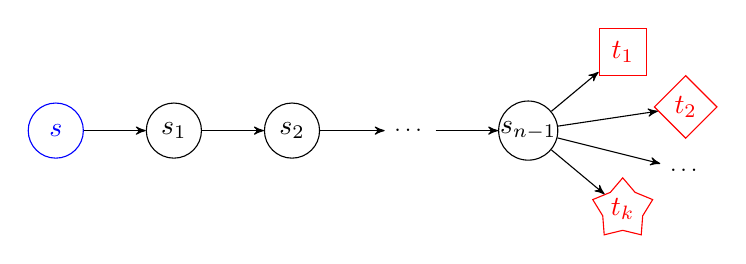
\begin{tikzpicture}
    \node[source]  (s)  at (0.0, 1) {$s$};
    \node[other]   (s1) at (1.5, 1) {$s_1$};
    \node[other]   (s2) at (3.0, 1) {$s_2$};
    \node[infobox] (sd) at (4.5, 1) {$\dots$};
    \node[other]   (sn) at (6.0, 1) {$s_{n-1}$};
    \node[target1] (t1) at (7.2, 2.0) {$t_1$};
    \node[target2] (t2) at (8, 1.3) {$t_2$};
    \node[infobox] (td) at (8, 0.5) {$\dots$};
    \node[targetk] (tk) at (7.2, 0.0) {$t_k$};

    \draw[->] (s)  -- (s1) node[midway] (ss1) {\phantom{0}};
    \draw[->] (s1) -- (s2) node[midway] (ss2) {\phantom{0}};
    \draw[->] (s2) -- (sd) node[midway] (ssd) {\phantom{0}};
    \draw[->] (sd) -- (sn) node[midway] (ssn) {\phantom{0}};
    \draw[->] (sn) -- (t1) node[midway] (st1) {\phantom{0}};
    \draw[->] (sn) -- (t2) node[midway] (st2) {\phantom{0}};
    \draw[->] (sn) -- (td) node[midway] (std) {\phantom{0}};
    \draw[->] (sn) -- (tk) node[midway] (stk) {\phantom{0}};
  \end{tikzpicture}
  \caption{An example where the $k$ search approach is inefficient.}
  \label{fig:k-search-bad}
\end{figure}
An extreme example of this inefficiency is depicted in Figure~\ref{fig:k-search-bad}.
The searched graph is a simple line ending with a star. % [[AF: maybe a fork?]].
In this case, \kxastar would generate $n$ nodes per sub-search, so it would generate $n + n + \dots + n = n\cdot k$ nodes in total, while it is easy to see that generating $n + k$ nodes is sufficient to solve this \kgs instance. %[[AF: problem appears twice]]
The ratio of node generations done by \kxastar to the number of node generations needed to solve this instance is $\frac{n\cdot k}{n + k}$ and can be made arbitrarily close to $k$.


More generally, this potential inefficiency of \kxastar stems from the fact that the searches do not share any information. To this end, we propose in the next section a \kgs algorithm that performs a single search towards all $k$ goals. Compared to \kxastar, this single search maintains one  \open and one \closed, thereby maximizing information reuse. We call this algorithm \kastar. 



\section{The \kastar Algorithm}
%\section{A Single Search for all  $k$ Goals}
\label{sec:one-k-goal-search}

Before presenting a complete pseudo code for \kastar, we highlight several aspects that differentiate it from \kxastar.

%needs to ... per node As a consequence of sharing \open and \closed, \kastar needs to ... per node. This value is based on the distance to start as well as all available heuristic information. 

\subsection{Maintaining the Set of Active Goals}

When a goal is expanded in \astar, the search halts.
By contrast, in \kastar the search does not halt until a lowest-cost path to each of the $k$ goals has been found.
To this end, \kastar tracks the set of goals that have not been expanded yet. 
We call $\activeg$ this set of \emph{active goals}.
%[[AF: use this term above when saying that a search notifies later search that their goal was found]].

%\subsection{Taking Advantage of the Heuristics}
\subsection{Guiding the Search with Multiple Heuristics}

%Say that a node $n$ is expanded by each of the $k$ \astar searches performed by \kxastar. Every search may assign a different heursitic value for $n$, since for every search the heuristic estimates the distance from $n$ to a different goal. That is, 
In \kxastar we implicitly assumed that for each goal $t_i$ there is a corresponding heuristic function $h_{t_i}$, so that $h_{t_i}(n)$ is the heuristic estimate of the cost to get from node $n$ to goal $t_i$. 


In \kastar, there is a single search, but we still have access to these $k$ heuristic functions. Formally, every generated node $n$ is associated with a $k$-ary vector $\vect{h}(n) = \tuple{h_{t_1}(n), \ldots h_{t_k}(n)}$. In \kastar, nodes ready to be expanded are prioritized based on their $g$ value, their $\vect{h}$ values, and the set of the active goals ($\activeg$). 

In more details, in every iteration \kastar selects from \open a node with the smallest $F$ value, which is computed by $F(n) = g(n) + \Phi_{\activeg}(\vect{h}(n))$, 
where $\Phi$ is a given aggregation function. 
The subscript $\activeg$ in $\Phi_\activeg$ denotes that the heuristic values for non-active goals (i.e., not in $\activeg$) are not aggregated.
This avoids  unnecessary computations when a node is generated. %, computing heuristics only for the active goals suffices to determine its $F$ value.
 
We discuss in Section~\ref{sec:aggregating} various design choices of  the heuristic aggregation $\Phi$, how they impact \kastar's behavior with respect to the properties of the given heuristic functions. % Nicer phrasing?
For now, assume the following natural instantiation of $\Phi$: 
\begin{equation}
\Phi_{\activeg}(\tuple{h_{t_1}(n), \dots h_{t_k}(n)}) = \min_{t_i\in\activeg} h_{t_i}(n) 
\label{eq:basic-phi-min}
\end{equation}
%and \[ \Phi_{\activeg}(\tuple{h_{t_1}(n), \dots h_{t_k}(n)}) = \max_{t_i\in\activeg} h_{t_i}(n) \]
%Meanwhile one can take $\Phi_{\activeg}(\tuple{h_{t_1}(n), \dots h_{t_k}(n)}) = \min_{t_i\in\activeg} h_{t_i}(n)$ or $\Phi_{\activeg}(\tuple{h_{t_1}(n), \dots h_{t_k}(n)}) = \max_{t_i\in\activeg} h_{t_i}(n)$ as reasonable instantiations. 



%Thus, the computational effort of generating a node in \kastar is larger than in regular \astar, as it requires computing $k$ heuristic values. 

%\footnote{As discussed later in the paper, the actual computational cost in \kastar can be smaller, since as the search progresses the list of relevant goals becomes smaller, and consequently computing $F$ becomes easier.}

%defining $\Phi[AG]$ as an aggregation function that only aggregates over the values that correspond to the set of goalsset $AG$ can accept vectors of different sizes, specifically any size between 1 and $k$, and only  Common aggregation functions such as $\max$, $\min$, and average are all such functions, as we can apply them to vectors of different sizes. 
%5[[TODO: New subsection to read]] Next, we ask the question of which heuristic aggregation functions can use Lazy \kastar and obtain  an admissible results (i.e., optimal paths to all goals). [[AF: I would summarize that eager and eager+ are always good. Lazy is OK for min but not for max. And now, we want to know what further with other functions]] To this end, we somewhat abuse [[AF: is this the correct word? You now use it on any size of vector up to k. Maybe you are widening it? Generalizing?]] the previous notation by defining $\Phi$ as an aggregation function that can accept vectors of different sizes,  specifically any size between 1 and $k$. % Common aggregation functions such as $\max$, $\min$, and average are all such functions, as we can apply them to vectors of different sizes. 




%\subsubsection*{Node evaluation function.} When searching for a single lowest-cost path with \astar, the state are popped from \open according to their $f=g+h$ values. In \kastar, we compute the $h$-value forand associate every state in \open with a value that considers the $h$-value for each of the $k$ goals.     Thus, when a state is generated then we compute the heuristic for each of the $k$ goals.


\begin{algorithm2e}
  \DontPrintSemicolon
  \KwIn{start $s$, goals $t_1, \ldots, t_k$}
  $g(s)\gets 0$; \open~$\gets \emptyset$; \closed~$\gets \emptyset$; \textsc{Solution}~$\gets \emptyset$\;
  \newcode{$\activeg$ $\gets \{t_1, \ldots, t_k\}$ \nllabel{line:init-active-goals}}\;
  \newcode{Add $s$ to \open with key $F(s) = g(s) + \Phi_{\activeg}(\vect{h}(s))$ \nllabel{line:computeF-start}}\;
  \While {\open $\neq \emptyset$} {
    $\mathit{best} \gets$ a node in \open with the smallest key \nllabel{kastar:line:open:chooseNode}\;
    Move $\mathit{best}$ from \open to \closed\;
    \newcode{
    \If {$\mathit{best}\in \activeg$}{
      \newcode{Add the path to $\mathit{best}$ to \textsc{Solution} \nllabel{line:storePath}}\;
      \newcode{Remove $\mathit{best}$ from $\activeg$ \nllabel{line:removeGoal}}\;
      \newcode{\For{every node $m$ in \open}{
        Update the key of $m$ to $F(m) = g(m) + \Phi_{\activeg}(\vect{h}(m))$ \nllabel{kastar:line:eager-update}
      }}
      \newcode{\lIf{$\activeg = \emptyset$}{
        \Return \textsc{Solution} \nllabel{kastar:line:allGoalsFound}}
      }
    }}
    \For{every outgoing edge $(\mathit{best}, c)$  \nllabel{kastar:line:nextNeighbor}}{
%      $c \gets $ generate a state by applying $A$ to $\mathit{best}$ \;
      $g_{new}\gets g(\mathit{best}) + w(\mathit{best}, c)$\;
      % Duplicate detection
      \If{$c \in$ \open $\cup$ \closed}{
        \lIf{$g(c) \leq g_{new}$}{
          \Continue (goto line~\ref{kastar:line:nextNeighbor})
        }
        Remove $c$ from \open and \closed
      }
      % Update n's g and f values
      $g(c)\gets g_{new}$ \\
      \newcode{Add $c$ to \open with key $F(c) = g(c) + \Phi_{\activeg}(\vect{h}(c))$ \nllabel{line:computeF}} \\
    }
  }
  \Return No solution exists \nllabel{kastar:line:noSolution}\\
  \caption{\kastar}
  \label{alg:kastar}
\end{algorithm2e}


Algorithm~\ref{alg:kastar} shows the pseudocode for \kastar. 
%We highlight the differences between the pseudo code of \astar (Algorithm~\ref{alg:astar}) and the pseudo code of \kastar (Algorithm~\ref{alg:kastar}) by marking every line that was changed or modified with a prefix ``[+]'' and the color blue. %[[AF: so many lines were changed so maybe just give the entire pseudo code. Everyone sees that it has a best-first search behavior]] 
Initially, all goals are inserted into the set of active goals, denoted  $\activeg$ (line~\ref{line:init-active-goals}).
Every node $n$ that is added to \open is associated with a $g$ value and a $F$ value.
Just like in \astar, the $g$ value of a node $n$ is the cost of a lowest-cost path found so far from the start $s$ to $n$.
The $F$ value is computed as $F(n) = g(n) + \Phi_{\activeg}(\vect{h}(n))$ as discussed above. 
The set of active goals $\activeg$ is needed to allow aggregating only the heuristics to these goals when computing the $F$ value, bypassing the need to compute the heuristics for the other goals. 
 
In every iteration, the node with the smallest $F$ value is selected and removed from \open (line~\ref{line:open:chooseNode}).
If it is a goal then we store the path to it (line~\ref{line:storePath}) and remove that goal from the active goal set $\activeg$ (line~\ref{line:removeGoal}).
Removing this goal from $\activeg$ marks that we are no longer looking for a path to that goal.
When this happens, we need to update the ordering of the nodes on \open (line~\ref{kastar:line:eager-update}).
When the $\activeg$ list is empty, we halt the search, having found a path to each goal.


% Completeness
\kastar returns \emph{no solution exists} only if \open is empty (line~\ref{kastar:line:noSolution}).
A node is removed from \open only after its children have been added to \open.
So, if \kastar reaches an iteration when \open is empty it means that some of the $k$ goals are not reachable.
Thus, \kastar is \emph{complete} in the sense that if it does not find a solution then indeed no solution exists.

\begin{proposition}[Completeness]
  \label{prop:completeness}
  If a goal is reachable, then it is eventually expanded by \kastar. 
\end{proposition}

% Soundness
\kastar halts and returns a solution after all $k$ goals have been expanded (line~\ref{kastar:line:allGoalsFound}).
When a state is expanded, it means a path to it has been found.
Thus, \kastar is \emph{sound}, in the sense that if it returns a solution then that solution contains a path from $s$ to each of the $k$ goals.
A key question is whether each of these $k$ paths is indeed an optimal path to its corresponding goal. 
In Section~\ref{sec:aggregating} we prove that 
using $\Phi$ as defined in Equation~\ref{eq:basic-phi-min} is \emph{admissible}, i.e., indeed leads to returning an optimal path for all goals. In addition, we define sufficient and necessary conditions for admissible aggregation functions, and suggest several alternatives aggregation function that satisfy these conditions. 

%[[AF: In line 23, don't you want to return some of the paths if you have them?]]\roni{I think this will just confuse. The problem is defined for all the $k$ paths.}

% What we have not described yet is how does the parallel search with a single \open aggregates the heuristic values for all goals, and how does the sequential searches choose which goal to solve first. In this work we focus on answering the first question.
%[[AF: This is indeed a summary and maybe it can be merged above somehow because there is repetition of text. Anyhow, it would be great to give a name to each of them or at least a sequential number.  And, there is a separation between everybody who only share information to KA* which uses one OPEN. This must be clear]]

\section{Aggregating Heuristic Values}
[[AF: some connecting sentences to tell me where I am??]]
\label{sec:aggregating}

We denote by \kastarphi the instantiation of \kastar that uses a given aggregation function $\Phi$. In the rest of this section, we examine under which assumptions on $\Phi$ and on the heuristics $\vect{h}$ we can obtain optimality guarantees on \kastarphi.
As we shall see, there is a tradeoff between the two types of assumptions: making stronger assumptions on the heuristics leads to a
larger class of aggregation functions that guarnatee optimality. %optimality for a larger range of aggregation functions. [[AF: not sure what the sentence means: it means optimallity]][[AS: Better now?]

Before analyzing the different aggregation functions and heuristics,  we provide the following definitions and invariant which holds in \kastar regardless of how the heuristics and $\Phi$ are computed.

\begin{definition}
  An algorithm for the \kgs is \emph{admissible} if in any instance, for all reachable goals $t_i$, the first path found to $t_i$ is optimal.
  An algorithm for the \kgs is \emph{$1$-admissible} if in any instance, there exists a goal $t_i$ such that the first path found to $t_i$ is optimal.
  [[Roni: do we need this 1-admissible? I rather we called this admissible]]
\end{definition}
\abda{check 1-admissible definition in case some goals are not reachable}

Since we defined \kgs for graphs with non-negative edge costs, we limit the discussion to non-negative heuristic functions and correspondingly heuristic aggregation functions that accept non-negative values. Formally,   
\begin{definition}
  Let $k$ be a fixed positive integer.
  A \emph{heuristic aggregation function} is a function $\Phi: \nonnegreals^k \rightarrow \nonnegreals$ such that $\Phi(\vect{0}) = 0$, where $\vect{0}$ is the $k$-dimensional zero vector.
\end{definition}

\begin{lemma}
  \label{lem:simple}
  In every iteration of \kastar, for every active goal $t_i$, there exists a state $n$ in \open on an optimal path to $t_i$, i.e., $g(n) + d(n, t_i) = d(s, t_i)$.
\end{lemma}

Lemma~\ref{lem:simple} can be proven by induction over the iterations of \kastar.
Namely, it trivially holds in the first iteration and continues to hold in subsequent iterations because when a node with $g(\cdot) + d(s,\cdot) = d(s, t_i)$ is expanded then one of its children must also have $g(\cdot) + d(s,\cdot) = d(s, t_i)$.
An equivalent to Lemma~\ref{lem:simple} has been proven for many other best-first search algorithms.

\begin{lemma}[Completeness]
  \label{lem:completeness}
  If a goal is reachable, then it is eventually expanded by \kastar. 
  %[[AF: but not necessarily optimal]
\end{lemma}
Note that Lemma~\ref{lem:completeness} does not say that the optimal path to each goal will be found. This requires some restrictions over the heuristics and aggregation function used, as we discuss next. 

\subsection{Consistent Heuristics}

We begin our exploration by considering the case where all heuristic functions are \emph{consistent} (Definition~\ref{def:consistent}). 


\begin{definition}
A heuristic aggregation function $\Phi$ is \emph{\axiomcons} iff for every vectors $\vect{v}$ and $\vect{u}$, we have that if there exists $i$ such that  $u_i = 0$ then $\Phi(\vect{v}) - \Phi(\vect{u}) \leq \max (\vect{v}-\vect{u})$.
\end{definition}
By $u_i$ we refer the $i^{th}$ element in $\vect{u}$. 

%\abda{Alternative names: \emph{metric}, \emph{weak contraction}. See \url{https://en.wikipedia.org/wiki/Metric_map} for inspiration.}
% Similar to \cite{Denardo1967}

\begin{theorem}
  \label{thm:consistent}
  Let $\Phi$ be a \axiomcons heuristic aggregation function.
  For any \kgs and for any tuple of consistent heuristics $\vect{h}$, \kastarphi is $k$-admissible.
\end{theorem}
\begin{proof}
  Assume that \kastar chooses to expand a goal $t_i \in \{t_1, \ldots t_k\}$) via a path $p$. 
  Applying Lemma~\ref{lem:simple} to $t_i$, we obtain there exists $n\in \open$ such that $g(n) + d(n, t_i) = d(s, t_i)$.
  Since $t_i$ is expanded before $n$, we have 
  \begin{equation}
      g(t_i) + \Phi(\vect{h}(t_i)) = F(t_i) \leq F(n) = g(n) + \Phi(\vect{h}(n))
  \end{equation}
    Since all heuristics are consistent, we have that for every $j$
  \begin{align}
    h_j(n)                  & \leq d(n, t_i) + h_j(t_i)   \\
    h_j(n) - h_j(t_i)       & \leq d(n, t_i)               
%    \Phi(\vect{h}(n)) - \Phi(\vect{h}(t_i)) & \leq d(n, t_i) & \text{($\Phi$ is \axiomcons and $h_i(t_i) = 0$)}\\
\end{align}
Since this holds for every $j$, we have: 
\begin{align}
    \max (\vect{h}(n) - \vect{h}(t_i)) & \leq d(n, t_i)              & \text{}\\
    \Phi(\vect{h}(n))-\Phi(\vect{h}(t_i))  & \leq d(n, t_i)  & \text{($\Phi$ is \axiomcons and $h_i(t_i) = 0$)}\\
        \Phi(\vect{h}(n))  & \leq d(n, t_i) + \Phi(\vect{h}(t_i)) & \\
    g(n) + \Phi(\vect{h}(n))           & \leq g(n)+ d(n, t_i) + \Phi(\vect{h}(t_i)) & \\
    F(n)           & \leq d(s, t_i) + \Phi(\vect{h}(t_i)) &
    \text{($n$ is chosen via Lemma~\ref{lem:simple})}
  \end{align}  
    Now, since $t$ is expanded before $n$, we have that $F(t_i) \leq F(n)$. 
  \begin{align}  
    F(t_i) \leq F(n)                     & \leq d(s, t_i) + \Phi(\vect{h}(t_i)) & \text{($t_i$ is expanded before $n$)}\\
    g(t_i) + \Phi(\vect{h}(t_i))           & \leq d(s, t_i) + \Phi(\vect{h}(t_i)) & \text{(by definition of $F$)}\\
    g(t_i)                & \leq d(s, t_i) & 
    \label{eq:consistent}
  \end{align}
  By definition of $d$, we know that $d(s,t_i)\leq g(t_i)$. Therefore, when we expand a goal its $g$ value is equal to $d(s, t_i)$ as required.
\end{proof}

Theorem~\ref{thm:consistent} shows that being \axiomcons is a sufficient condition for optimality of \kastarphi with consistent heuristics.
Our next result shows that it is a necessary condition. 
\begin{figure}
  \centering
  \subfloat{
  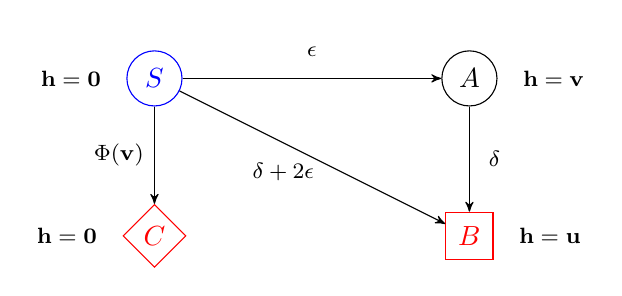
\begin{tikzpicture}
    \node[source] (s) at (0, 2) {$S$};
    \node[other]  (a) at (4, 2) {$A$};
    \node[target1] (b) at (4, 0) {$B$};
    \node[target2] (c) at (0, 0) {$C$};

    \draw[->] (s) -- (a) node[midway] (sa) {\phantom{0}};
    \draw[->] (s) -- (b) node[midway] (sb) {\phantom{0}};
    \draw[->] (s) -- (c) node[midway] (sc) {\phantom{0}};
    \draw[->] (a) -- (b) node[midway] (ab) {\phantom{0}};

    \node[above = -2mm of sa,edgeweight] {$\epsilon$};
    \node[below left = -5mm of sb,edgeweight] {$\delta + 2\epsilon$};
    \node[left  = -2mm of sc,edgeweight] {$\Phi(\vect{v})$};
    \node[right = -2mm of ab,edgeweight] {$\delta$};

    \node[left  = 2mm of  s,infobox] {$\vect{h}=\vect{0}$};
    \node[right = 2mm of  a,infobox] {$\vect{h}=\vect{v}$};
    \node[right = 2mm of  b,infobox] {$\vect{h}=\vect{u}$};
    \node[left  = 2mm of  c,infobox] {$\vect{h}=\vect{0}$};
  \end{tikzpicture}
  } \hfill
  \subfloat{
    \begin{tabular}[b]{lccc}
      \toprule
      Path & $g$ & $\Phi(\vect{h})$ & $F$\\
      \midrule
      $SB$ & $\delta + 2\epsilon$ & $\Phi(\vect{u})$ & $\Phi(\vect{v}) - \epsilon$ \\
      $SC$ & $\Phi(\vect{v})$ & $0$ & $\Phi(\vect{v})$\\
      $SA$ & $\epsilon$ & $\Phi(\vect{v})$ & $\Phi(\vect{v}) + \epsilon$ \\
      $SAB$ & $\delta + \epsilon$ & $\Phi(\vect{u})$ & $\Phi(\vect{v}) - 2\epsilon$ \\
      \bottomrule
    \end{tabular}
  }
  \caption[Generic counter-example for \kastarphi]{Generic counter-example for \kastarphi. 
  The start is $S$, $B$ is the $i$\textsuperscript{th} goal, and $C$ is the $j$\textsuperscript{th} goal for $j \neq i$. 
  For any, $\vect{v}$, $\vect{u}$, $i$, $\delta$, and $\epsilon$ such that (1) $u_i = 0$, (2) $\delta > 0$, (3) $\Phi(\vect{v}) > \Phi(\vect{u}) + \delta$, and (4) $\epsilon = \frac{\Phi(v) - \Phi(\vect{u}) - \delta}{3} > 0$, running \kastarphi will return a suboptimal path to $B$. 
  
  To see this, the table on the right shows the $g$, $\Phi(\vect{h})$, and $F$ values for the possible paths to the graph nodes.
  The search expands $S$, $B$, $C$, then stops.
  The optimal path to $B$ is $SAB$, but \kastarphi returns the suboptimal path $SB$.}
  \label{fig:kstarphi-bad}
\end{figure}
\begin{theorem}
  \label{thm:consistent-dual}
  If a heuristic aggregation function $\Phi$ is not \axiomcons, then there exists a \kgs and a tuple of consistent heuristics such that \kastarphi is not $k$-admissible.
\end{theorem}
\begin{proof}
Since $\Phi$ is not \axiomcons, there exists vectors $\vect{v}$, $\vect{u}$, and an index $i$ such that $u_i = 0$ and $\Phi(\vect{v}) - \Phi(\vect{u}) > \max (\vect{v} - \vect{u})$. 
  Let $\delta$ such that $\Phi(\vect{v}) - \Phi(\vect{u}) > \delta > \max (\vect{v} - \vect{u})$.
Since the domain of $\Phi$ is vectors of non-negative values, $v_i \geq 0$ and so $\max (\vect{v} - \vect{u}) \geq v_i - u_i \geq 0$, therefore $\delta > 0$.


  Define $\epsilon = \frac{\Phi(\vect{v}) - \Phi(\vect{u}) - \delta}{3} > 0$.
  Using $\vect{v}$, $\vect{u}$, $i$, $\delta$, and $\epsilon$, we can construct a counter-example showing that \kastarphi is not $k$-admissible. 
  This counter example is given in Figure~\ref{fig:kstarphi-bad}. 
$S$ is the start, $B$ is the $i$\textsuperscript{th} goal and $C$ is the $j$\textsuperscript{th} goal for $j \neq i$. 
     As can be seen from the table above right, the search expands $S$, $B$, $C$, then stops. 
     The optimal path to $B$ is $SAB$, but \kastarphi returns the suboptimal path $SB$. 

  To conclude the proof, it remains to observe that the heuristics involved are consistent.
  This is indeed the case because for all $j$, we have $h_j(A) - h_j(B) = v_j - w_j \leq \max (\vect{v} - \vect{w}) < \delta = d(A, B)$ and therefore $h_j(A) \leq d(A, B) + h_j(B)$.
\end{proof}

[[UP TO HERE 19.10]]

Theorem~\ref{thm:consistent} opens the opportunity to run \kastar for a larger range of heuristic aggregation functions than Theorem~\ref{thm:admissible}, provided the heuristic functions are consistent.

\begin{observation}
  Any \axiomadm function is also \axiomcons.
%  In particular $\Phi=\min$ is \axiomcons.
\end{observation}
\begin{proof}
  Let $\Phi$ be an \axiomadm heuristic aggregation function and let $\vect{v}$ and $\vect{w}$ be vectors such that $\exists i, w_i = 0$.
  On the one hand, $\Phi(\vect{v}) - \Phi(\vect{w}) \leq \Phi(\vect{v}) \leq \min \vect{v} \leq v_i$.
  On the other hand, we have $w_i = 0$ so we derive $v_i \leq v_i - w_i \leq \max (\vect{v} - \vect{w})$.
  As result, $\Phi(\vect{v}) - \Phi(\vect{w}) \leq \max (\vect{v} - \vect{w})$, and we conclude that $\Phi$ is \axiomcons.
\end{proof}

Let $\{ v_i \}$ be a collection of terms. [[AF: what does that mean? numbers? Who is i? do you have vi, v2 etc?]][[AF: do you want to start a new definition here?]]
A \emph{subconvex} combination of these terms is a linear combination $\sum_i \alpha_i t_i$ where all coefficients are non-negative, $0 \leq \alpha_i$, and the sum of coefficients is no more than one, $\sum_i \alpha_i \leq 1$.

The $i$th \emph{order statistic} of a vector $\vect{v}$ is the $i$th smallest value of $\vect{v}$ and is denoted $v_{(i)}$. [[AF: why not just call it i'th smallest?]
For instance, if $\vect{v} = \tuple{3, 1, 0, 1}$, then $v_{(1)} = v_3 = 0$, $v_{(2)} = v_{(3)} = v_2 = v_4 = 1$ and $v_{(4)} = v_1 = 3$. [[AF: this is just a permutation along the values]

[[AF: jumped further. I am happy to sit down with whoever wrote this to further polish the text]

The \axiomcons axiom is not only as general as \axiomadm, but it also allows for aggregation functions not covered by the previous assumption:
\begin{theorem}
  \label{thm:subconvex}
  Subconvex combinations of the components and the order statistics give rise to \axiomcons heuristic aggregation functions.
\end{theorem}
\begin{proof}
  Consider $2k$ non-negative coefficients $\alpha_i$ such that $\sum_{1 \leq i \leq 2k} \alpha_i \leq 1$.
  Then, we will show that $\Phi$ defined as $\Phi(\vect{v}) = \sum_{1 \leq i \leq k} \alpha_i v_i + \alpha_{k+i} v_{(i)}$ is a heuristic aggregation function.
  For any two vectors $\vect{v}$ and $\vect{w}$, we have $\Phi(\vect{v}) - \Phi(\vect{w}) = \sum_{1 \leq i \leq k} \alpha_i (v_i - w_i) + \alpha_{(i+k)} (v_{(i)} - w_{(i)})$.
  On the one hand, $v_i - w_i \leq \max (\vect{v} - \vect{w})$ is direct, on the other hand, $v_{(i)} - w_{(i)} \leq \max (\vect{v} - \vect{w})$ can be established with a little bit more effort:

  Indeed, for $1 \leq i \leq k$, define $V_i = \{j, v_j < v_{(i)} \}$ and $W_i = \{j, w_j < w_{(i)} \}$ and observe that $|V_i| \leq i - 1$ and $|W_i| \leq k - i$ by definition of the order statistics.
  It follows that $|V_i \cup W_i| \leq k - 1$.
  From a counting argument, obtain an integer $1 \leq l_i \leq k$ such that $l_i \notin V_i \cup W_i$.
  By construction of $V_i$ and $W_i$, deduce that $v_{(i)} \leq v_{l_i}$ and that $w_{l_i} \leq w_{(i)}$ and conclude that $v_{(i)} - w_{(i)} \leq v_{l_i} - w_{l_i} \leq \max (\vect{v} - \vect{w})$.

  As a result, we have $\Phi(\vect{v}) - \Phi(\vect{w}) \leq \sum_{1 \leq i \leq 2k} \alpha_i \max(\vect{v} - \vect{w})$ because for all $i$, $\alpha_i$ is non-negative.
  Therefore, $\Phi(\vect{v}) - \Phi(\vect{w}) \leq \max(\vect{v} - \vect{w}) \sum_i \alpha_i \leq \max(\vect{v} - \vect{w})$, thus showing that $\Phi$ is \axiomcons.
\end{proof}

\begin{corollary}
  Using any of the \emph{mean}, the \emph{maximum}, the \emph{minimum}, the \emph{$i$th projection}, for $1 \leq i \leq k$, or the \emph{median} of the values in $\vect{v}$ gives a \axiomcons heuristic aggregation function.
\end{corollary}
\begin{proof}
  All these quantities can be expressed as subconvex combinations of the components and the order statistics, so they are all \axiomcons:
  The $i$th projection is $\Phi(\vect{v}) = v_i$; the \emph{mean} is $\Phi(\vect{v}) = \frac{v_1 + \dots + v_k}{k}$; the \emph{maximum} is $\Phi(\vect{v})= v_{(k)}$; the \emph{minimum} is $\Phi(\vect{v}) = v_{(1)}$; and the \emph{median} is $\Phi(\vect{v}) = \frac{1}{2}(v_{(\frac{k}{2})} + v_{(\frac{k+1}{2})})$.
\end{proof}

It is easy to show that for $2 \leq k$, none of these heuristic aggregation function is \axiomadm, except for the \emph{minimum}.
Thus, Theorem~\ref{thm:consistent} does indeed extend the range of functions for which we can obtain guarantees to other natural aggregation methods.

\begin{observation}
  The following heuristic aggregation functions do not satisfy \axiomcons.
  The \emph{sum} aggregation, $\Phi(\vect{v}) = \sum_i v_i$ is not \axiomcons as soon as there are two goals or more.
  More generally, combinations of the components that are not subconvex do \emph{not} give rise to \axiomcons heuristic aggregation functions.
\end{observation}
\begin{proof}
  Consider non-negative coefficients $\alpha_i$ such that $\sum_i \alpha_i > 1$.
  Then, $\Phi$ defined as $\Phi(\vect{v}) = \sum_i \alpha_i v_i$ is a heuristic aggregation function.
  However, taking for instance $\vect{v} = \vect{1}$ and $\vect{w} = \vect{0}$, we have $\vect{v} - \vect{w} = \sum_i \alpha_i (1 - 0) = \sum_i \alpha_i > 1 = \max (\vect{v} - \vect{w})$.
  Therefore $\Phi$ is not \axiomcons.
  In particular, the sum aggregation function is not \axiomcons.
\end{proof}

\begin{observation}
  The \emph{range statistic}, $\Phi(\vect{v}) = v_{(k)} - v_{(1)}$, is \axiomcons.
  For $k \geq 3$, the ``almost-range'' statistic defined as $\Phi(\vect{v}) = v_{(k)} - v_{(2)}$ is not \axiomcons.
\end{observation}
\begin{proof}
\abda{blabla}
\end{proof}

%\subsection{blabla}

\begin{theorem}
  \label{the:kastarmin-surplus}
  For any \kgs and for any tuple of consistent heuristics $\vect{h}$, \kastarmin never expands a surplus state.
\end{theorem}
\begin{proof}
  Let $n$ be a node expanded by \kastarmin.
  Let $t_i$ be such that $h_{t_i}(n) = \min h_{t_i}(n)$.
  Applying Lemma~\ref{lem:simple} to $t_i$, we obtain $n_i \in \open$ such that $g(n_i) + d(n_i, t_i) = d(s, t_i)$.
  For any node $p$ on the path from $s$ to $n$, we have the following derivation.
  \begin{align}
    h_{t_i}(p)        & \leq d(p, n) + h_{t_i}(n)         & \text{($h_{t_i}$ is consistent)}\\
    h_{t_i}(p)        & \leq d(p, n) + \Phi(\vect{h}(n))         & \text{(from the choice of $t_i$)}\\
    g(p) + h_{t_i}(p) & \leq g(p) + d(p, n) + \Phi(\vect{h}(n)) & \text{}\\
    g(p) + h_{t_i}(p) & \leq g(n) + \Phi(\vect{h}(n))          & \text{Lemma blabla}\\
    g(p) + h_{t_i}(p) & \leq F(n)         & \text{(by definition of $F$)}\\
    g(p) + h_{t_i}(p) & \leq F(n_i) = g(n_i) + \Phi(\vect{h}(n_i))      & \text{($n$ is expanded)}\\
    g(p) + h_{t_i}(p) & \leq g(n_i) + h_i(n_i) & \text{(by definition of $\Phi$)}\\
    g(p) + h_{t_i}(p) & \leq g(n_i) + d(n_i, t_i) & \text{($h_{t_i}$ is admissible)}\\
    g(p) + h_{t_i}(p) & \leq d(s, t_i) & \text{($n_i$ is chosen via Lemma~\ref{lem:simple})}
    \label{eq:nosurplus}
  \end{align}
  Thus, $n$ is not surplus for the SPP $\Pi_i$.
  Therefore, $n$ is not surplus for the \kgs.
\end{proof}

Note that our assumption that $h_{t_1}, \ldots h_{t_k}$ are consistent is necessary for the proof of Theorem~\ref{the:kastarmin-surplus}.
With an admissible but inconsistent heuristic, \kastarmin may, in fact, expand surplus states.
Figure~\ref{fig:inconsistent} shows a \kgs problem with $k = 2$ where this occurs.
\kastarmin will expand all states in the figure, while $B$ is surplus for both goals.

\begin{figure}
%  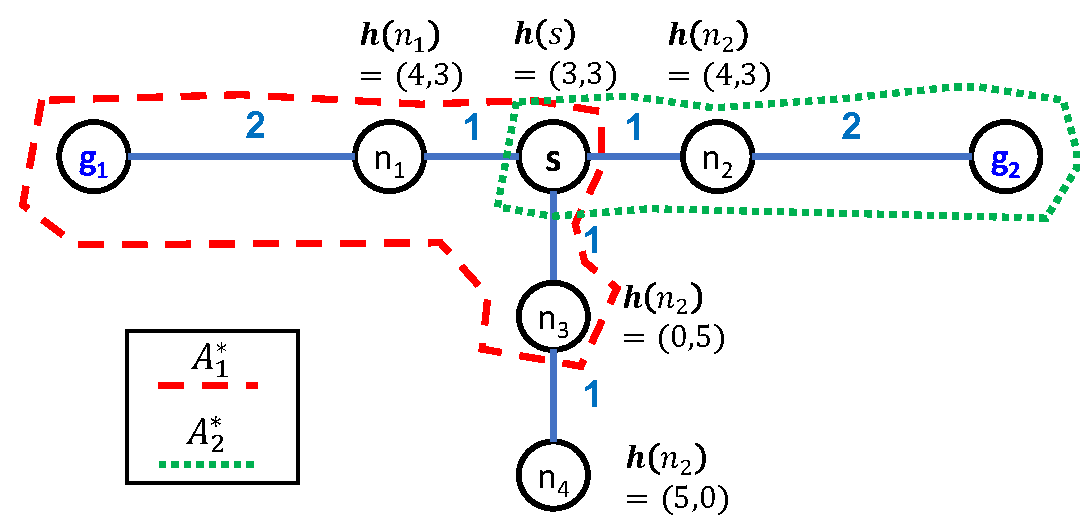
\includegraphics[width=\columnwidth]{inconsistent_cropped.pdf}
  \subfloat{
    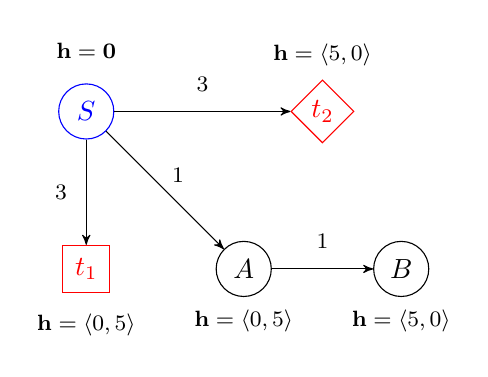
\begin{tikzpicture}
    \node[source]  (s)  at (0, 2) {$S$};
    \node[other]   (a)  at (2, 0) {$A$};
    \node[other]   (b)  at (4, 0) {$B$};
    \node[target1] (t1) at (0, 0) {$t_1$};
    \node[target2] (t2) at (3, 2) {$t_2$};

    \draw[->] (s) -- (a)  node[midway] (sa) {\phantom{0}};
    \draw[->] (a) -- (b)  node[midway] (ab) {\phantom{0}};
    \draw[->] (s) -- (t1) node[midway] (st1) {\phantom{0}};
    \draw[->] (s) -- (t2) node[midway] (st2) {\phantom{0}};

    \node[above right = -5mm of sa,edgeweight] {$1$};
    \node[above = -2mm of ab,edgeweight] {$1$};
    \node[left  = -2mm of st1,edgeweight] {$3$};
    \node[above = -2mm of st2,edgeweight] {$3$};

    \node[above = 1mm of  s,infobox] {$\vect{h}=\vect{0}$};
    \node[below = 0mm of  a,infobox] {$\vect{h}=\tuple{0, 5}$};
    \node[below = 0mm of  b,infobox] {$\vect{h}=\tuple{5, 0}$};
    \node[below = 1mm of  t1,infobox] {$\vect{h}=\tuple{0, 5}$};
    \node[above = 0mm of  t2,infobox] {$\vect{h}=\tuple{5, 0}$};
  \end{tikzpicture}
  } \hfill
  \subfloat{
    \begin{tabular}[b]{l*8{c}}
      \toprule
      \multirow{2}{*}{Path} &     & \multicolumn{2}{c}{\astari{t_1}} & \multicolumn{2}{c}{\astari{t_2}} & \multicolumn{3}{c}{\kastarmin} \\
      \cmidrule(r){3-4} \cmidrule(lr){5-6} \cmidrule(l){7-9}
              & $g$ & $f$ & S  & $f$ & S  & $\Phi(\vect{h})$ & $F$ & S \\
      \midrule
      $S$    & $0$ & $0$ & \xmark & $0$ & \cmark & $0$ & $0$ & \xmark \\
      $St_1$ & $3$ & $3$ & \xmark & $8$ & \cmark & $0$ & $3$ & \xmark \\
      $St_2$ & $3$ & $8$ & \cmark & $3$ & \xmark & $0$ & $3$ & \xmark \\
      $SA$   & $1$ & $1$ & \xmark & $6$ & \cmark & $0$ & $1$ & \xmark \\
      $SAB$  & $2$ & $7$ & \cmark & $2$ & \cmark & $0$ & $2$ & \cmark \\
      \bottomrule
    \end{tabular}
  }
  \caption{An example where \kastarmin expands a surplus state, $B$.
    The table on the right indicates which nodes are expanded and whether the corresponding state is surplus ($S$) for \astari{t_1}, \astari{t_2}, and \kastarmin.
    This example relies on the inconsistency of the second heuristic: $h_{t_2}(A) >  d(A, B) + h_{t_2}(B)$.
  }
  \label{fig:inconsistent}
\end{figure}

An equivalent theorem for \kastarmax does not hold.
Indeed, there are cases where \kastarmax expands surplus states.
For example, consider the \kgs problem in Figure~\ref{fig:lazy}.
State $A$ will be expanded first, having $F_{\max}(A) = 4$, followed by $t_2$ ($F_{\max}(t_2) = 10$)), and finally $t_1$ ($F_{\max}(t_1) = 11$).
However, neither \astari{1} nor \astari{2} will expand $A$.
Moreover, $A$ is surplus w.r.t. both $\Pi_1$ and $\Pi_2$, since the optimal path to $t_1$ and $t_2$ costs 3 and 1, respectively, while $f_1(A) = 4 > 3$ and $f_2(A) = 2 > 1$.



==========================================






\subsection{General Heuristic Aggregation Functions}
The operators $\min$ and $\max$ are two ways to aggregate the heuristic values of a given node, but \kastar can also be implemented with other aggregation functions, functions that accept a vector of $k$ values and output a single value.
\begin{definition}
  Let $k$ be a fixed positive integer.
  A \emph{heuristic aggregation function} is a function $\Phi: \nonnegreals^k \rightarrow \nonnegreals$ such that $\Phi(\vect{0}) = 0$, where $\vect{0}$ is the $k$-dimensional zero vector.
\end{definition}
\kastar can use such a function to computes the $F$ value of a node $n$, as $F(n) = g(n) + \Phi(\vect{h}(n))$, where $\vect{h}(n)$ is the vector $\tuple{h_1(n), h_2(n), \dots, h_k(n)}$.
We denote the resulting algorithm as \kastarphi.
%Such a heuristic aggregation function accepts a vector of $k$ heuristic values of a node  and outputs a single value, which is then used by \kastar to compute node's $F$ value.  Formally,

In the rest of this section, we examine under which assumptions on $\Phi$ and on the heuristics $\vect{h}$ we can obtain optimality guarantees on \kastarphi.
As we shall see, there is a tradeoff between the two types of assumptions.
Making stronger assumptions on the heuristics leads to optimality for a larger range of aggregation functions. [[AF: not sure what the sentence means: it means optimallity]][[AS: Better now?]



\subsection{Admissible Heuristics}
\begin{definition}
  A heuristic aggregation function $\Phi$ is \emph{\axiomadm} iff for every vector $\vect{v}$, we have $\Phi(\vect{v}) \leq \min \vect{v}$.
\end{definition}
[[AF: adm-compat???]]
\begin{observation}
  $\Phi = 0$ and $\Phi=\min$ are \axiomadm.
\end{observation}

\begin{theorem}
  \label{thm:admissible}
  Let $\Phi$ be a \axiomadm heuristic aggregation function.
  For any \kgs and for any tuple of admissible heuristics $\vect{h}$, \kastarphi is $k$-admissible.
\end{theorem}
\begin{proof}
  Assume that \kastarphi chooses to expand a goal $t_i\in\{t_1,\ldots t_k\}$.
  Applying Lemma~\ref{lem:simple} to $t_i$, we obtain $n\in \open$ such that $g(n) + d(n, t_i) = d(s, t_i)$.
  Since $t_i$ is expanded before $n$, we have $g(t_i) + \Phi(\vect{h}(t_i)) = F(t_i) \leq F(n) = g(n) + \Phi(\vect{h}(n))$.

  \begin{align}
    h_{t_i}(n) & \leq d(n,t_i) & \text{($h_{t_i}$ is admissible)}\\
    \Phi(\vect{h}(n)) \leq \min_{t_j} h_{t_j}(n) & \leq d(n, t_i) & \text{($\Phi$ is \axiomadm)}\\
    g(n) + \Phi(\vect{h}(n)) & \leq g(n) + d(n, t_i) = d(s, t_i) & \text{($n$ is chosen via Lemma~\ref{lem:simple})}\\
    F(t_i) \leq F(n) & \leq d(s, t_i) & \text{($t_i$ is expanded before $n$)}\\
    g(t_i) + \Phi(\vect{h}(t_i)) & \leq d(s, t_i) & \text{(by definition of $F$)}\\
    g(t_i) & \leq d(s, t_i) & \text{($\Phi$ is non-negative)}\\
    d(s, t_i) \leq g(t_i) & \leq d(s, t_i) & \text{(by definition of $d$)}
%    \label{eq:admissible}
  \end{align}
  Therefore, when we expand a goal its $g$ value is equal to $d(s,t_i)$ as required.
\end{proof}

Theorem~\ref{thm:admissible} shows that being \axiomadm is a sufficient condition for optimality of \kastarphi with admissible heuristics.
Our next result shows that it is a necessary condition.

\begin{theorem}
  \label{thm:admissible-dual}
  If a heuristic aggregation function $\Phi$ is not \axiomadm, then there exists a \kgs and a tuple of admissible heuristics such that \kastarphi is not $k$-admissible.
\end{theorem}
\begin{proof}
  Let $\vect{v}$ such that $\Phi(\vect{v}) > \min \vect{v}$.
  Let $\vect{w} = \vect{0}$, $i = \argmin \vect{v}$, and $\delta$ such that $\Phi(\vect{v}) > \delta > \min \vect{v} = v_i$.
  Note that $\Phi(\vect{v}) > \Phi(\vect{w}) + \delta$ and consider the counter-example in Figure~\ref{fig:kstarphi-bad}.

  To conclude the proof, it remains to observe that the heuristics involved are admissible.
  This is indeed the case because we have $h_{t_i}(A) \leq \min \vect{v} \leq \delta = d(A, B)$ and therefore $h_{t_i}(A) \leq d(A, B)$.
\end{proof}

[[AF: doesn't this mean that MIN is the only reasonable function that is k-admissible? Anything smaller than min is not reasonable in my option. It is like cutting a heuristic down]

\begin{theorem}
  \label{the:kastarmin-surely}
  Let $\Phi$ be a \axiomadm heuristic aggregation function. For any \kgs and for any tuple of admissible heuristics $\vect{h}$, \kastarphi expands all the surely expanded nodes.
\end{theorem}
\begin{proof}
%  Consider the \open and \closed lists when the last goal is expanded.
  Let $n$ be a node that is surely expanded w.r.t. some goal $t_i$.
  That is, $n$ is reachable from $s$ by a path of nodes with $f_i$ values lower than $d(s, t_i)$ and $f_i(n) < d(s, t_i)$.
  $\Phi$ is \axiomadm so for any node $m$ along this path we have $\Phi(m) \leq \min_{t_j} h_{t_j}(m) \leq h_{t_i}(m)$.
  Thus, the $F$ values of the nodes along this path must also be lower than $d(s, t_i)$.
  As all edges in the underlying graph have non-negative cost, $h_{t_i}(t_i) = 0$ and therefore $F(t_i) = d(s, t_i)$.
  Hence, the minimal $F$ value in \open is $d(s, t_i)$ when $t_i$ is expanded.
  Thus, all the nodes along the path to $n$ and $n$ itself must have already been expanded, as all of them have $F$ values smaller than $d(s, t_i) = F(t_i)$.
\end{proof}


\subsection{Arbitrary Heuristics}
%\abda{$\Phi$ needs to be constant $0$.}

\begin{definition}
  \label{def:ucs}
  \ac{kUCS} is the \kastarvar{0} algorithm where the heuristic aggregation function is the constant 0 function which maps any vector to value 0.
\end{definition}
\ac{kUCS} runs a best-first search without a heuristic, prioritizing nodes based on their $g$ values alone, basically running Dijkstra's algorithm~\cite{DIJ59,Felner2011}, until all goals are expanded.  %As a result, UCS finds the optimal path to every reachable state, including every reachable goal---it is $k$-admissible.

\begin{theorem}
  \label{thm:arbitrary}
  For any \kgs instance and for any tuple of heuristics, \ac{kUCS} is $k$-admissible.
\end{theorem}

\ac{kUCS} does not use any heuristic information and is guaranteed to find the optimal path for each goal. However, without imposing any restriction on the heuristic functions, \ac{kUCS} is the only \kastar instantiation that is $k$-admissible with arbitrary heuristics. 
For example, let $k=1$ and assume that the heuristic functions is inadmissible. Clearly, \kastar will return a suboptimal solution. We 

\begin{theorem}
  \label{thm:arbitrary-dual}
  If a heuristic aggregation function $\Phi$ is not the constant 0, then there exists a \kgs instance and a tuple of arbitrary heuristics such that \kastarphi is not $k$-admissible.
\end{theorem}
\begin{proof}
  $\Phi$ is not the constant function 0, so there exists a vector $\vect{v}$, such that $\Phi(\vect{v}) > 0$,
  Let $\vect{w} = \vect{0}$, $i = 1$, and $\delta$ such that $\Phi(\vect{v}) > \delta > 0$.
  Note that $w_i = 0$ and that $\Phi(\vect{v}) > \Phi(\vect{w}) + \delta = \delta$ and consider the counter-example in Figure~\ref{fig:kstarphi-bad}. [[AF: not clear what are the different variables? nodes? just variables? Also, I think the text in the caption should be placed in the main text]][[AF: I suggest to move all the vector from bold to a letter with a bar above or bellow]]
\end{proof}





%In \astar{} for a single goal, states are prioritized in \open according to the $f=g+h$ value of a state. In contrast, a state in \kastar{} has a vector of $k$ heuristic values $\vect{h}(n)$ and consequently a vector of $f$ values $\vect{f}$(n) that contains one $f$ value per goal. Therefore, \kastar{} requires a state evaluation function that aggregates these $f$ values in some way. In Algorithm~\ref{alg:k-goal-bfs} this is encapsulated in the {\tt ComputeF} function. We refer to the value ($F$) returned by this function as the state's $F$ value, and consider the following two options for computing it.
We consider the following two options for computing the $F$ value of a state:  
\begin{align}
  \text{\minf} =& g(n) + \min_{i\in [1,k]}h_i(n) \\
  \text{\maxf} =& g(n) + \max_{i\in [1,k]}h_i(n)
\end{align}
\kastar that uses \minf as the state evaluation function is referred to hereinafter as \kastarmin, and similarly \kastar that uses \maxf is referred to as \kastarmax. [[AF: If this was not already defined earlier then put this earlier. No need to re-define]]





%[[AF: I do not like the term maxf and do not like that you say that it is admissible without exactly defining what you mean. Can you omit this and only talk on kastarmax]]\roni{Fixed}. [[ARIEL UP TO HERE]]

[[AF: maybe we just talk on the general case first and then mention that max and min are special cases?]]


[[AF: again, some connecting sentences can help out here]]




\section{Maintaining \open in \kastar}
\label{sec:lazy}

For the rest of this paper, we assume that we use an admissible combination of heuristics and heuristic aggregation function.
In other words, either, the heuristics are consistent and $\Phi$ is \axiomcons, or the heuristics are admissible and $\Phi$ is \axiomadm, or the heuristics are arbitrary and $\Phi$ is the constant 0.
%[[AF: then why above did you also assume inconsistent. Maybe assume this for the entire paper and delete everything that has to do with inconsistent heuristics. The paper is too long with details anyway.]]
Thus, according to Theorems~\ref{thm:consistent} and~\ref{thm:admissible}, when a goal $t_i$ is expanded by \kastarphi we are guaranteed that the optimal path to it has been found.
%[[AF: both only mentioned above but not yet defined and the terms were not yet defined and used. Theorems 16 and 18 were not yet given. Try to re-word or to bring the necessary definitions before this claim (or move this to afterwards]]
This allows us to safely remove $t_i$ from the set of active goals (see line~\ref{line:removeGoal} in Algorithm~\ref{alg:kastar}).
Not only does removing a goal from the set of active goals affect as only heuristics for the remaining active goals will be considered.
This has an impact on how the $F$ values is computed in subsequent \kastar iterations, but it also affect the $F$ value of nodes currently in \open.

\subsection{The need for recomputations}
Intuitively, several nodes may have had a high priority in \open solely because they were estimated to be close to goal $t_i$.
After $t_i$ is expanded, it may very well be preferable not to prioritize these nodes anymore.
Thus, in principle, a node in \open may be associated to an \emph{up-to-date} or to a \emph{stale} $F$ value, depending on whether it has been recomputed based on the latest set of active goals $\activeg$. 
Line~\ref{kastar:line:eager-update} in Algorithm~\ref{alg:kastar} ensures that every node in \open is always mapped to the most up-to-date $F$ value.
% [[AF: you must reorder OPEN now]]

On the one hand, traversing and re-ordering \open every time a goal is expanded can incur a significant overhead.
On the other hand, skipping any sort of $F$ value update could result in an inefficient algorithm because the stale $F$ values provide poor guidance to the search, directing it towards goals that are no longer active.

For example, consider the \kgs depicted in Figure~\ref{fig:lazy} and assume that we use $\Phi = \min$ as the heuristic aggregation function. %[[AF: just fully define Fmin and Fmax above.]]
%The edge weights are depicted next to the edges.
The shortest paths to $t_1$ and $t_2$ do not go through any other intermediate node and cost 3 and 1 respectively.
After $S$ is expanded, the nodes in \open are $t_2$, $A$, $t_1$, and $C$, in that order, with $F$ values as given in the table (column $F_{t_1,t_2}$).
Thus, $t_2$ is expanded next.
This goal expansion should trigger a reordering of \open according to line~\ref{kastar:line:eager-update}.
Let us examine, however, what happens if this step is omitted and if the search is allowed to continue with stale $F$ values.
In that case, \open would contain the nodes $A$, $t_1$, and $C$, in that order, and with stale keys as described in the table (column $F_{t_1,t_2}$).
So $A$ would be expanded, followed by expanding $t_1$ and halting.

On the other hand, if the $F$ values are recomputed after $t_2$ is not an active goal anymore, then \open would contain the nodes $t_2$, $A$, and $C$, in that order and with up-to-date keys as described in the table (column $F_{t_1}$).
Using these up-to-date $F$ values, $t_1$ is expanded after $t_2$ and then the search halts, returning the optimal paths to $t_1$ and $t_2$ without ever expanding neither $A$ nor $C$.
Both of which are surplus nodes with respect to both $t_1$ and $t_2$ (Definition~\ref{def:surplus}).
Thus, considering stale $F$ values can introduce inefficiency to the search and lead to the unnecessary expansion of surplus nodes, here $A$.

%[[AF: nice example. But, the text has too much past tense "would have been etc". Try to simplify the text]]


\begin{figure}
  \centering
  \subfloat{
    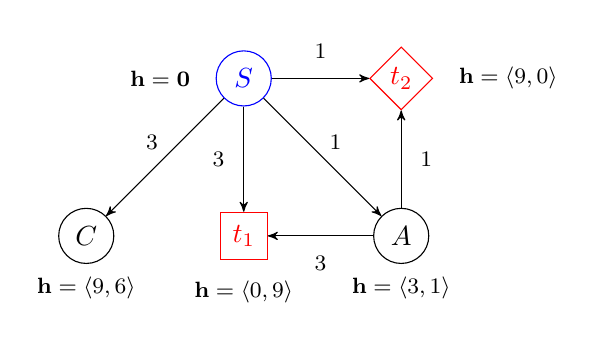
\begin{tikzpicture}
    \node[source]  (s)  at (2, 2) {$S$};
    \node[other]   (a)  at (4, 0) {$A$};
    \node[target2] (t2) at (4, 2) {$t_2$};
    \node[other]   (c)  at (0, 0) {$C$};
    \node[target1] (t1) at (2, 0) {$t_1$};

    \draw[->] (s) -- (a)  node[midway] (sa) {\phantom{0}};
    \draw[->] (s) -- (t2)  node[midway] (st2) {\phantom{0}};
    \draw[->] (s) -- (c)  node[midway] (sc) {\phantom{0}};
    \draw[->] (s) -- (t1) node[midway] (st1) {\phantom{0}};
    \draw[->] (a) -- (t1) node[midway] (at1) {\phantom{0}};
    \draw[->] (a) -- (t2) node[midway] (at2) {\phantom{0}};

    \node[above right = -5mm of sa,edgeweight] {$1$};
    \node[above left = -5mm of sc,edgeweight] {$3$};
    \node[left  = -2mm of st1,edgeweight] {$3$};
    \node[below = -2mm of at1,edgeweight] {$3$};
    \node[above = -2mm of st2,edgeweight] {$1$};
    \node[right = -2mm of at2,edgeweight] {$1$};

    \node[left  = 2mm of  s,infobox] {$\vect{h}=\vect{0}$};
    \node[below = 0mm of  a,infobox] {$\vect{h}=\tuple{3, 1}$};
    \node[below = 0mm of  c,infobox] {$\vect{h}=\tuple{9, 6}$};
    \node[below = 1mm of  t1,infobox] {$\vect{h}=\tuple{0, 9}$};
    \node[right = 2mm of  t2,infobox] {$\vect{h}=\tuple{9, 0}$};
  \end{tikzpicture}
  } \hfill
  \subfloat{
    \begin{tabular}[b]{lccccc}
      \toprule
      Path & $g$ & $\Phi_{t_1, t_2}(\vect{h})$ & $F_{t_1, t_2}$ & $\Phi_{t_1}(\vect{h})$ & $F_{t_1}$\\
      \midrule
      $St_2$  & $1$ & $0$ & $1$ & & \\
      $SA$    & $1$ & $1$ & $2$ & $3$ & $4$\\
      $St_1$  & $3$ & $0$ & $3$ & $0$ & $3$\\
      $SAt_1$ & $4$ & $0$ & $4$ & $0$ & $4$\\
      $SAt_2$ & $2$ & $0$ & $2$ & & \\
      $SC$    & $3$ & $6$ & $9$ & $9$ & $12$\\
      \bottomrule
    \end{tabular}
  }
  \caption[Illustrating the pitfalls of not reordering \open.]{Example illustrating the pitfalls of not reordering \open, using $\Phi = \min$.
  Running \kastarmin without reordering \open after a goal is expanded (i.e., omitting line~\ref{kastar:line:eager-update} from Algorithm~\ref{alg:kastar}) results in expanding a surplus state ($A$).

  Running Lazy \kastarmin recomputes the value of $A$ after expanding $t_2$, but avoids expanding $A$; Lazy \kastarmin does not recompute the value of $C$.}
  \label{fig:lazy}
\end{figure}

For the sake of disambiguation, we will refer to the baseline approach displayed in Algorithm~\ref{alg:kastar} as \emph{Eager} \kastarphi instead of just \kastarphi.
Using Eager \kastar can be costly, as it requires reordering \open $k-1$ times. 
We analyze the runtime overhead induced by these reorderings in Section~\ref{sec:resource-analysis}.

In the rest of this Section, we describe two variants of \kastarphi that perform fewer $F$ value recomputations than the Eager \kastarphi without expanding any additional node.
These variants are called \emph{Reactive} \kastarphi and \emph{Lazy} \kastarphi.

%sec:smart-eager

\subsection{Reactive \kastarphi}
\label{sec:reactive}
%One option to avoid using stale $F$ values is to completely reorder \open after removing a goal from the set of active goals (line~\ref{line:removeGoal}).
%This is done by re-computing the node evaluation function for all nodes in \open to get their up-to-date $F$ value, and then reordering \open accordingly.
%We refer to this option as \emph{Eager \kastar}. %[[AF: I of course like the name. Again, use other names for the other variants above.]]


Observe that the $F$ value of some states does not become stale when a goal is removed from the set of active goals.
For example, consider a \kgs instance with 3 goals and a state $n$ with $f$ values $\vect{f}(n)= \tuple{10, 5, 3}$.
When using \kastarmin, $F(n)=f_3(n)=3$.
Therefore, the $F$ value of $n$ will only change if the goal $t_3$ is removed from the set of active goals.
In particular, the $F$ value of $n$ does not become stale when either $t_1$ or $t_2$ are removed from the set of active goals, as this does not change the (up-to-date) $F$ value of $n$. [[AF: You might want to say that if F=3 then the paths to the other nodes was found with $f \leq 3$ and this is why this node is still in OPEN]]
Consequently, there is no point in to re-computing $F(n)$ when goal $t_1$ or $t_2$ are expanded. More generally, after a goal $t_i$ is expanded there is no need to re-compute the $F$ value of a state if it is not stale  [[AF: there is a need to recompute only for stale nodes]]. %that iof any state for which $F(n)\neq f_i(n)$.
%expanded there is no need to re-compute the $F$ value of any state for which $F(n)\neq f_i(n)$.

\begin{definition}
Let $\Phi$ be a heuristic aggregation function, let $\activeg$ be a set of active goals, and let $n$ be a node.
A set of goals $\respog \subseteq \activeg$ are \emph{responsible} for $n$, w.r.t. $\activeg$, if for any set of goals $\activeg'$ such that $\respog \subseteq \activeg' \subseteq \activeg$, we have that $\Phi_{\respog}(\vect{h}(n)) \leq \Phi_{\activeg'}(\vect{h}(n)) \leq \Phi_{\activeg}(\vect{h}(n))$.
\end{definition}

Typically, there are multiple sets of responsible goals, starting with $\activeg$.
We may choose one arbitrarily, but in principle, it is always better to focus on a minimal set of responsible goals (i.e., such that there are no strict subset that would also be responsible).
Furthermore, in practice it is often better to focus on a minimum set of responsible goals (i.e., such that there any other set of responsible goals has greater or equal cardinality).
%[[AF: how about principal goal? or key goal?]] [[AS: not "key" because we use this term in the context of \open being ordered by keys (the F values).]]

[[AS: give example using min]]

We implemented this optimization by storing additional information for each node $n$, keeping track of the goal $t_i$ for which $F(n)=f_i(n)$.
We refer to this goal as the \emph{responsible goal} of $n$.
If there are multiple responsible goals, we choose one arbitrarily.
%[[AF: Why? choose them all. Only when it is empty you should re-order open]]
Then, we re-compute the $F$ value of a node and re-insert [[change its priority]] it into \open only if one of its responsible goals is no longer active.
%[[AF: if you have two responsible goals and one is removed there is no need to recalculate its value. Of course, you will need to store a list of responsible goals. In fact, you can store a vector of $k$ bits and set the ones that are responsible. Only when this vector is all 0 you need to recalculate the $F$-value. Outch, this is the version below]][[Roni and Meir: we only keep one responsible node. One could keep a list of responsible, but that seems overly complex. Meir might try anyhow to implement this]]
This version of \kastarphi is referred to as Reactive \kastarphi.
%[[AF: I would not call it eager+. This is an implementation trick for eager and should not have its own sign.]] [[AF: you do not only recompute. You also change its place in \open. If there are too many of these, why not sort \open from scratch?]]

%Note that if a 
A more involved implementation would keep track of all the sets of responsible goals for every node.
%I.e., storing for every node $n$, the set of goals for which $f(n)=F(n)$.
Then, when a goal $t_i$ is expanded, we iterate over every node that had $t_i$ in its set of responsible goals and remove $t_i$ from that set.
Then, a state will only re-compute its $F$ value (and re-position it in \open accordingly) if its set of responsible goals is empty.
This approach, however, requires storing more information per state and is more complex, and so we implemented only Eager$^+$ in our experimental evaluation (Section~\ref{sec:experimentalResults}). [[AF: call the new one Eager++?]] %[[AF: OK, you answered me. But, I think this should be the correct way to do eager. I do not like eager+ not in its name and not in its content. By the end of the day, the responsible goal is out of the computation so it does not really matter.]]
%former approach, which keeps track of a single responsible goal.

%[[AF: the last sentence is not understandable. you keep the set for who? Which nodes? For everybody? please better explain what you mean. I did not understand. Also, consider to delete this all together. You did not implement it so why bother? Maybe in a footnote? But, please better explain for sure.]]

%[[AF: I would delete all the non eager+ from the experiments]]

% Lazy!

[[ARIEL GOT HERE. 24/06/18 at 17:05]]

\subsection{Lazy \kastar}
% We outlined above an example where the cost of reordering \open after a goal is expanded does not [[AF: I think you want to delete the "not"]]incur significant overhead [[AF: where did you outline this? You just showed that you must reorder open, otherwise, you have more node expansions]]. However, this is not always the case. For example, in domains where the search frontier does not grow exponentially, then states generated after the $k-1$ goal has been expanded are not larger than the states generated up to that point. Indeed, we show in our experimental results that in some domains reordering does, in fact, incur a significant amount of runtime.
%[[AF: you just said that it is negligible. Please explain why this is not the case in these domains. Are they polynomial?]]

%[[AF: Roni will reword and say that eager can be costly.]]

Both Eager \kastar and Reactive \kastar will re-compute the $F$ value and reinsert [[AF: reorder is used when the entire list is reoredered. You mean that we will have to apply some kind of change-priority for these nodes. Minor issue.]] all the states in \open that have stale $F$ values.
This incurs a cost that can be significant, as we observed in our experimental evaluation.
To this end, we propose an alternative approach in which states are re-evaluated and reinserted in \open in a lazy manner.
This means we re-compute a state's $F$ value only if at least one of its responsible goals is not active \emph{and} it is selected for expansion (line~\ref{line:open:chooseNode} in Algorithm~\ref{alg:kastar}).
Then, we re-insert it into \open only if its $F$ value has increased and it no longer has the minimal $F$ value in \open.


We call this algorithm Lazy \kastar, since it is directly inspired by the Lazy \astar algorithm~\cite{betzalel2015typeSystem,tolpin2013toward}, where multiple heuristics are used towards the same goal, and are evaluated lazily in a similar manner.
Lazy \kastar behaves differently when using \maxf than when using \minf. [[AF: never defined]]
Thus, we analyze them separately.
%[[AF: I already said that I think these terms are redundant. Your call]]\roni{I don't see a better way to discuss the different F functions then to name them}

%n particular, the lazy approach only brings benefit to \kastarmin

\subsubsection{Lazy \kastarmin}

Consider running Lazy \kastarmin [[AF: also never defined]] on the graph depicted in Figure~\ref{fig:lazy}.
Lazy \kastarmin behaves exactly as Eager \kastarmin until the first goal is expanded, which in this case is $t_2$.
At this stage, \open contains $t_1$, $A$, and $C$ with $F$ values 3, 2, and 9, respectively.
The $F$ values of $A$ and $C$ are stale, and therefore Eager$^+$ \kastarmin (and also Eager \kastarmin) will re-compute their $F$ values and re-insert them into \open.
Lazy \kastarmin does not do so.
Instead, it continues with these stale $F$ values, selecting $A$ from \open.
Lazy \kastarmin then observes that $F(A)$ is stale and re-computes it.
The updated $F$ value of $A$ is 4, which is greater than the $F$ value of $t_1$, 3.
So, $A$ is re-inserted into \open and the next state selected from \open is $t_1$.
After expanding $t_1$ the search halts, having an optimal path to both goals.
As we can see, Lazy \kastarmin did not re-compute the $F$ value of $C$ although it was stale.
Nonetheless, Lazy \kastarmin did not expand more states than Eager \kastarmin.

More generally, the following Lemma shows that although Lazy \kastarmin does not reorder all the states in \open when a goal is expanded and thus its \open may contain states with stale $F$ values,
it still manages to expand states in order of their up-to-date $F$ values. % (i.e., according to the $F^u$ value).

%This occurs not just in this example, but in generalWe now prove this observation to the  that this is true not just in this example but in general.

% As a result, $n_2$  and re-position it in \open so that the  Note that the responsible goal for $n_3$ is $g_2$, so when $g_2$ is expanded both Eager \kastarmin and Eager$^+$ \kastarmin will re-compute the $F$ value of $n_3$ (updating it to 16) and re-position it in \open accordingly. Running Lazy \kastarmin will not do so, since  i \kgs our running example from Figure~\ref{fig:need-resort}.  Lazy \kastarmin behaves exactly as Eager \kastarmin until the first goal is expanded, which in this case is $g_2$. Recall that at this stage \open consists $g_1$ and $n_2$, having $\textbf{f}(g_1)=(6,15)$ and  $\textbf{f}(n_2)=(7,5)$. Since $g_1$ and $n_2$ were inserted into \open when both $g_1$ and $g_2$ were active, their $F$ values are $F(g_1)=6$ and $F(n_2)=5$. Both $F$ values are stale, as  if we computed them now (after $g_2$ was removed from the set of active goals), we will have $F(g_1)=6$ and $F(n_2)=7$. Using Eager (or Eager), and are thus stale,  since $g_2$ is now removed from the set of active goals and thus  $F_min().
%We now prove that although Lazy \kastarmin does not reorder all the states in \open when a goal is expanded, it still expands states in order of their up-to-date $F$ values. % (i.e., according to the $F^u$ value).
% Lazy with minf is good
\begin{lemma}[Lazy \kastarmin is a best-first search]
Lazy \kastarmin always expands the state in \open with the smallest up-to-date $F$ value. % $F^u$
%Every path $\pi_i$ returned by Lazy \kastarmin is guaranteed to be the lowest-cost path to its corresponding goal ($g_i$).
\label{the:lazy-minf-correct}
\end{lemma}
\begin{proof}

%[[AF: the same sentence is repeated three times.]]
At a given point in time, a state $n$ may have a stale $F$ value (according to which it is positioned in \open), and an up-to-date $F$ value.
To differentiate between them, we denote the former by $F(n)$ and the latter by $F^u(n)$.
Lemma~\ref{the:lazy-minf-correct} thus states that if $n$ is expanded by Lazy \kastarmin then $F(n)=\min_{n'\in \open}F^u(n')$. [[Define this once and present the lemma only once; no need for repetition]]
We prove this by induction on the iterations of the main loop of Lazy \kastarmin.
%, showing that Lazy \kastarmin and Eager \kastarmin expand exactly the same set of states.
The base of the induction is trivial: in the first step $F(s)=F^u(s)$ and \open contains only $s$.
Now assume that in the first $m-1$ iterations, Lazy \kastarmin expanded the state with the smallest $F^u$ value, and consider the $m^{th}$ iteration of Lazy \kastarmin.

First, observe that $F(n)\leq F^u(n)$ [[AF: I would write: $F^u(n)\geq F(n)$ ]for every state $n$.
This is because the $F$ value in \kastarmin is the minimum over the $f$ values for the active goals and the set of active goals when $F$ was computed is either the same or a superset of the current set of active goals (according to which $F^u(n)$ is computed).

Now, let $n$ be the state selected for expansion from \open in the $m^{th}$ iteration of Lazy \kastarmin. Hence, it had the smallest $F$-value in \open.
In addition, $F(n)=F^u(n)$, as otherwise it would have been re-inserted into \open.
Therefore
%\[ \forall n'\in\open ~~ F^u_{min}(n)=F_{min}(n)\leq F_{min}(n') \leq F^u_{min}(n') \]
\[ \forall n'\in\open ~~ F^u(n)=F(n)\leq F(n') \leq F^u(n') \]
  So, $n$ has the smallest $F^u$ value in \open, as required.
\end{proof}

[[AF: proof is trivial. You might want to omit it to gain space]

The implication of Lemma~\ref{the:lazy-minf-correct} is that both Lazy \kastarmin and Eager \kastarmin expand states according to their $F^u$ values, except that Lazy \kastarmin does so more efficiently, without the need to reorder all the stale states in \open.
% [[AF: So you do reorder the entire open list. with Eager. Or do you only insert these nodes that their F values was changed?]]

However, the exact sets of states they expand may be different due to tie breaking.
For example, consider a tie-breaking rule that chooses the state that has the smallest sum of $f$ values (among the states with the same $F$ value).
Now, assume that we have two states in \open, $n_1$ and $n_2$, with $\mathbf{f}$ values $\tuple{5, 6, 10 }$ and $\tuple{5, 7, 7}$, respectively.
They have the same $F$ value (5), but according to this tie-breaking rule \kastarmin will choose $n_2$ before $n_1$.
Now, assume that $t_3$ was expanded.
Using Eager \kastarmin would result in $n_1$ now being expanded before $n_2$, while Lazy \kastarmin would not do so.
Since tie-breaking rules can make a significant difference in performance~\cite{asai2017tieBreaking}, this means that Eager \kastarmin may still outperform Lazy \kastarmin.
In our experimental results, however, this did not occur and Lazy \kastarmin was in general better. %[[AF: Tie breaking can go either way. You might want to delete all this altogether]]\roni{I don't follow}

[[AF: Tie breaking can go either way. That is, tie breaking can favor each of them and probably on average does not favor anyone more than the other. Thus, you might want to delete this discussion all this altogether, as tie breaking did not provide any surprising experimental results.]]
% Lazy does not work for Max-f, but  does work on Min-f
\subsubsection{Lazy \kastarmax}

%Using Lazy \kastarmin has significant impact [[AF: what do you mean, runs faster? explain why?]] in practice. Unfortunately,
Lemma~\ref{the:lazy-minf-correct} does not transfer to Lazy \kastarmax.
%Using the Lazy approach for \kastarmax does not have the same effect.
In fact, we show next that Lazy \kastarmax is equivalent to running \kastarmax that does not reorder \open when a goal is expanded.
This results in Lazy \kastarmax expanding states with stale $F$ value, even if there are other states in \open whose up-to-date $F$ values are smaller.
%In fact, Lazy \kastarmax is equivalent to running \kastarmax without reordering \open after a goal is expanded.
%,and thus it may expand states that do not have the lowest updated $F$ value in \open.
%[[AF: who is not doing the reordering. Ambiguous. Please precisely say what you mean]].
%[[AF: recall? I do not remember anything??]]
As discussed above (and shown in the example in Figure~\ref{fig:lazy}), this is a negative result since it means that Lazy \kastarmax will be guided towards goals even after the optimal path to them has been found.
[[AF: so this algorithm is no-good and should not be used. Do you want to prove theorems on that?]]
% we cannot apply the lazy approach to \kastarmax and preserve admissibility.
\begin{theorem}%[Lazy \kastarmax is not a best-first search]
  Lazy \kastarmax expands exactly the same set of states as \kastarmax, without reordering \open.
  \label{the:lazy-maxf-bad}
\end{theorem}

[[Delete the comma. Also, I think that you can call it by name KA*MAX-Basic or something similar. It is very confusing to jump between variants the way you do it]]

\begin{proof}
  To prove Theorem~\ref{the:lazy-maxf-bad}, we show that if Lazy \kastarmax selects a state from \open it will never decide to insert it back in \open.
  Let $n$ be a state with the minimal $F$ value in \open.
  Lazy \kastar decides to re-insert $n$ iff both conditions hold: (1) $F(n)$ is stale, and
  (2) there is a state $n'$ in \open for which $F(n')<F^u(n)$. %whose $F$ value is smaller than the up-to-date $F$ value of $n$.
  Assume, by negation, that such a state $n'$ exists.
  Since $n$ was selected for expansion before $n'$, we have that $F(n)\leq F(n')$.
  Now, observe that when using \maxf to compute $F$ values, then $F^u(m)\leq F(m)$ for every state $m$.
  Thus, $F^u(n)\leq F(n) \leq F(n')$, contradicting the assumption that $F(n')<F^u(n)$.
\end{proof}
%Consider Figure~\ref{fig:lazy}(a). First $s$ is expanded, generating $n_1$ and $n_2$ with ${\textbf{f}}(n_1)=(10,3)$  and ${\textbf{f}}(n_2)=(7,7)$. Thus, $n_2$ will be expanded, generating $g_1$ and $g_2$, each with a $g$ value of 7.  Assume that the heuristic of $g_1$ and $g_2$ are both zero (for both goals). Then \kastarmax will expand next $g_1$ and $g_2$, never expanding $n_1$ and returning a suboptimal path to $g_2$ of cost 7.

[[AF: ]The main point is that with MAX the f-value can only go down and this will not push it deeper into open.]]

% Using Lazy \kastarmin has significant impact in practice, as it decides in many cases to re-insert into \open the state with the minimal $F$ value. This is not the case in Lazy \kastarmax. In fact, Lazy \kastarmax will \emph{never} re-insert a state into \open after re-computing its $F$ value.
%To better understand why Lazy \kastarmax This is because re-computing an $F$ value for a state after the set of relevant goals has been reduced will only cause the $F$ value to decrease. Thus, is a state already has the smallest $F$ value in \open, it will still have the smallest $F$ value after we re-compute its $F$ value.
For this reason, we implemented only the two Eager approaches (Eager and Eager$^+$) for \kastarmax.

%[[AF: not clear. You never used lazy? What two approaches. This entire section needs some more rewording as I said. I think I do want to see this section 5 again.]]

%[[AF:  As I said above, I think we only need eager and the exact implementation is less important. That is, I do not like the term eager+. Your call]]


\subsubsection{Lazy for General Aggregation Functions}
[[TODO: New subsection to read]]
Next, we ask the question of which heuristic aggregation functions can use Lazy \kastar and obtain  an admissible results (i.e., optimal paths to all goals). [[AF: I would summarize that eager and eager+ are always good. Lazy is OK for min but not for max. And now, we want to know what further with other functions]]
To this end, we somewhat abuse [[AF: is this the correct word? You now use it on any size of vector up to k. Maybe you are widening it? Generalizing?]] the previous notation by defining $\Phi$ as an aggregation function that can accept vectors of different sizes,  specifically any size between 1 and $k$.
Common aggregation functions such as $\max$, $\min$, and average are all such functions, as we can apply them to vectors of different sizes. 

\begin{definition}
We say that a heuristic aggregation function $\Phi$ is \emph{isotone} if for any two sets $\activeg' \subseteq \activeg$ and for any vector $\vect{v}$, it holds that $\Phi_{\activeg'}(\vect{v})\leq \Phi_{\activeg}(\vect{v})$.
Conversely, $\Phi$ is called \emph{antitone} if $\Phi_{\activeg'}(\vect{v})\geq \Phi_{\activeg}(\vect{v})$ for any sets $\activeg'\subseteq \activeg$ and vector $\vect{v}$.
\end{definition}

%[[AF: you mean that with a subset it never gets larger. The term "monotonically" usually means that as time passes and something progresses. Here, you delete items. So, maybe use a different term. Something from set theory. I do not have anything in mind. Maybe reverse the term: if when adding more items you may get a smaller value you are monotonically non-increasing and vise versa]][[AS: How about now?]]

The $\min$ and $\max$ operators are trivial examples of, respectively, antitone and isotone aggregation functions.
%[[AF: add that Max and Min are trivial examples of non-increasing/]]
%We now provide sufficient conditions for identifying an aggregation function that can be used with Lazy \kastar, and when these conditions results in an effective use of Lazy \kastar.
\begin{theorem}
  If a heuristic aggregation function $\Phi$ is antitone then Lazy \kastarphi always expands the state with the smallest up-to-date $F$ value.
\end{theorem}
\begin{proof}
Let $\Phi$ be an antitone heuristic aggregation function, $n$ be a node chosen for expansion, and $n'$ be some other node in \open.
Now, assume that the $F$ value of $n'$ was computed w.r.t. a set of active goals $\activeg$ and that the current set of active goals is $\activeg'\subset \activeg$.

Node $n$ is chosen for expansion so its $F$ value is up-to-date, so $F(n)=g(n)+\Phi_{\activeg'}(\vect{h}(n))$, and also the smallest in \open, so $F(n)\leq F(n')=g(n')+\Phi_{\activeg}(\vect{h}(n'))$.
Since $\Phi$ is antitone, $F(n')\leq F^u(n')$, as required.  [[AF: intuitively, for a subset of goals the aggregated value can on only increase so choosing it now as the minimal node in open is safe.]]
\end{proof}

\begin{observation}
  \label{obs:genMaxNoLazy}
  If a heuristic aggregation function $\Phi$ is isotone then Lazy \kastarphi expands exactly the same set of nodes as \kastarphi without reordering \open.
\end{observation}
Observation~\ref{obs:genMaxNoLazy} is a straightforward generalization of Theorem~\ref{the:lazy-maxf-bad},
since for every $n$ having the minimal $F$ value and a set of active goals $\activeg$ and its subset $\activeg'$ it holds that $F(n)=g(n)+\Phi_{\activeg}(\vect{h}(n))\geq g(n)+\Phi_{\activeg'}(\vect{h}(n))=F^u(n)$. 

[[AF: say a few words about eager?]]

[[AF: also I am wondering whether there are better functions than min?]]



%\section{Theoretical Analysis of the Resource Usage}
\section{Resource Analysis}
%\section{State, Memory, and Time Complexities}
\label{sec:resource-analysis}
% Analysis

In this section we compare analytically the two main approaches we proposed for the \kgs problem: $k$ searches for one goal (\kxastar) or one search for $k$ goals (\kastar).

\subsection{Expanded States}
\label{sec:expandedStates}

[[AF: what about new variants that came out from the previous section][]

First, we analyze the set of states expanded by the two approaches.
We denote by Exp(\astari{i}), Exp(\kxastar), Exp(\kastarmin), and Exp(\kastarmax), the sets of states expanded by \astari{i} (for a given $i$), \kxastar, \kastarmin, and \kastarmax, respectively.
It is easy to see that
\begin{equation}
  \text{Exp}(\text{\kxastar})=\cup_{i=1}^k \text{Exp}(\text{\astari{i}})
\end{equation}
Note that Exp($X$) is the \emph{set} of states that were expanded, and not the number of state expansions.
In particular, if a state is expanded twice then it shall appear in Exp($X$) only once. ]]AF: why would that happen? Because of regular inconsistencies or because of something specific to the new algorithms?]]

To analyze the relationship between Exp(\kxastar), Exp(\kastarmin), and Exp(\kastarmax), we use the notion of surplus and surely expanded states for \kgs problems (Definition~\ref{def:surplus-k-goal}) and the corresponding results for \kxastar and \kastar (Proposition~\ref{prop:kxastar-effective}, Theorem~\ref{the:kastarmin-surely}, and Theorem~\ref{the:kastarmin-surplus}).
The practical implication of these results is that, as long as the heuristics are consistent, \kastarmin and \kxastar expand the same set of states up to tie breaking.
The notion of ``up to tie breaking'', however, is problematic in this context, since ties in \kastarmin refer to states with the same $F$ value while ties in \kxastar refer to states with the same $f_i$ value for some particular goal $t_i$.
Nonetheless, for ease of presentation, we will make the simplifying assumption hereinafter that \kxastar and \kastarmin expand the same set of states.


[[AF: I do not see any analysis here. You just define the notions. Also, you did not use the terms of surplus must-expand etc.]]

%because comparing \kastarmin and \kxastar, since ties in \kastarmin refer to states with the same $F$ value while ties in \kxastar refer to states with the same $f_i$ value for some particular goal $g_i$.


% Memory=generated
\subsection{Memory Requirements}
The number of states expanded is directly related to the number of generated states,\footnote{If $b$ is the branching factor then there are $b$ times more generated states than expanded states.} which in turn is related to the memory requirements of \astar and \kastar.
In general, search algorithms that store all the generated states in \open and in \closed, such as \astar and \kastar, are memory intensive.
While other implementations are also possible, where only the states in \open and their predecessors are stored~\cite{zhou2006breadth,korf2004best} or where the states are stored in external memory~\cite{zhou2004structured,edelkamp2016external,edelkamp2005external}, we focus our analysis on the more common implementation of \astar in which all generated states are stored in memory for the entire duration of the search.

Hence, the memory required for the algorithms discussed in this paper is proportional to the number of (distinct) states generated times the memory required to store a single state.
%Without loss of generality, assume that each state requires one memory units to store and denote by Gen($X$) the set of states generated by algorithm $X$. From Observation~\ref{obs:expandedStates}, we can bound the memory required to run \kastarmin as follows:
In our analysis we make the simplifying assumption that each state requires one memory unit to store for all algorithms.\footnote{This assumption is not exactly correct in practice, since in \kastar we store for a state a vector of $k$ values ($\vect{f}(n)=\tuple{f_1,\ldots,f_k}$) while in \astar we only store a single value.
Nonetheless, we justify our assumption for cases where the memory required to store the state details is significantly larger than these $k$ values.  [[AF: hard point to sell. But, maybe it is more than just a footnote?]]}
Hence, if Mem($X$) and Gen($X$) denotes the memory required and the set of states generated when running algorithm $X$, respectively, then, up to tie-breaking between states with the same $F$ value, it holds that:
\begin{align}
Mem(\text{\kxastar})&=\max_{j\in [1,k]}| Gen(\text{\astari{j}})| \label{eq:kxastar-mem}\\
Mem(\text{\kastarmin})&=|\bigcup_{j\in [1,k]} Gen(\text{\astari{j}})| \label{eq:kastar-mem}\\
Mem(\text{\kxastar})&\leq Mem(\text{\kastarmin}) \leq \sum_{j\in[1,k]} Mem(\text{\astari{j}}) \label{eq:kxastar-kastar-mem}
\end{align}

The correctness of Equations~\eqref{eq:kxastar-mem}--\eqref{eq:kxastar-kastar-mem} is now established.
Since \kxastar runs the $k$ searches independently, there is no need to store the states generated by \astari{i} when running \astari{j}.
Thus, to run \kxastar we require memory sufficient to run each \astari{i} individually (Equation~\eqref{eq:kxastar-mem}).
In \kastarmin we expand the same set of states as \kxastar and thus generate the same set of states, but we must store them throughout the search.
Thus, \kastar stores every state $n$ that is  generated by one of the $k$ searches in \kxastar, i.e., the union $\bigcup_{j\in[1,k}Gen(\text{\astari{j}})$ (Equation~\eqref{eq:kastar-mem}).
The size of this union cannot be smaller than the cardinality of the set of stated generated by any individual \astar, but cannot be larger than their sum (Equations~\eqref{eq:kxastar-kastar-mem}).
Note that these bounds [[AF: which bounds? do you mean that $\leq$ is not $<$]are tight, in the sense that there are $k$-goal problems where $Mem(\text{\kxastar}) = Mem(\text{\kastarmin})$ and other $k$-goal problems where $Mem(\text{\kastarmin}) = \sum_{j\in[1,k]} Mem(\text{\astari{j}})$.
For example, in a 2-goal instance, if $Gen(\text{\astari{1}})\subset Gen(\text{\astari{2}})$ then $Mem(\text{\kxastar}) = Mem(\text{\kastarmin})$ while if $Gen(\text{\astari{1}})\cap Gen(\text{\astari{2}})=\{s\}$ then $Mem(\text{\kastarmin}) = \sum_{j\in[1,k]} Mem(\text{\astari{j}})-1$, where the minus one is for the start state. %[[AF:Except for the start state]]

[[]All the above discussion is relatively trivial but is nice to have]]


\subsection{Runtime Analysis}

Now we analyze the expected runtime of the proposed \kgs algorithms. [[AF: you only do this for two of them. Also, which variant do you talk about eager? Lazy? etc][]
As shown above theoretically and will be shown later experimentally, \kastarmin is almost always superior to \kastarmax, and thus the focus of our analysis is a comparison between \kxastar and \kastarmin (denoting the latter as simply \kastar throughout this section). 
While both algorithms generate the same set of states, % (Theorem~\ref{the:expanded-equal}),
their runtimes differ due to the number of times each state is generated and the cost of these generations.



%%%%%%%%%%%%%%%%%%%%%%%%%%%%%
\subsubsection{Runtime of \kxastar}
To analyze the runtime of \kxastar, consider the operations performed by an \astar search whenever a state is generated (lines~\ref{line:astar:generate-start}--\ref{line:astar:generate-end} in Algorithm~\ref{alg:astar}):

\begin{enumerate}
  \item \textbf{Generation}  (lines~\ref{line:astar:generate-start}--\ref{line:dd-end} and \ref{line:astar:generate-end}).
  This refers to computing the generated state by applying an action to the expanded state, performing duplicate detection (updating the $g$ value to the generated if needed), and inserting the generated state to \open (if needed).
  We denote the computational cost of this step as $C_{gen}$.

  \item \textbf{Heuristic computation}  (lines~\ref{line:computeF-start} and~\ref{line:computeF}).
  This refers to computing the $h$ value of the generated state.
  We denote the computational cost of this step as $C_{h}$.
\end{enumerate}

The exact value of $C_{gen}$ depends on the domain and various implementation details, such as the data structure used to implement \open and the state representation.
In the textbook implementation of \astar on simple domains, \open is implemented as a Binary heap and the domain actions are easy to compute and so $C_{gen}$ is linear in the size of a state's representation in memory and (plus) logarithmic in the size of \open (the cost of inserting an item in a Binary heap).
But faster implementations are also possible in some domains, where adding to \open incurs a constant time~\cite{GILON2016,BurnsHLR12}.
Similarly, the cost of the heuristic computation ($C_h$) can vary widely as well, where some heuristics require constant time to compute while more sophisticated heuristics may involve poly-time computations or even worse.


%Each of these operations incur some computational cost. Let $C_{gen}, C_{dd}, C_{h},$ and $C_{add}$ denote the average computation cost of the above four operations, generation, duplicate detection, heuristic computation, and insertion into \open, respectively. In addition,

%[[AF: either the i is a subscript or in brackets. Standardize.]]
We perform our runtime analysis with respect to the above cost model, which assumes that $C_{gen}$ and $C_h$ are approximately constant for all states.
Under this assumption, the runtime of \kxastar is straightforward.
\[
Time(\text{\kxastar}) = \sum_{i\in[1,k]} |Gen(\text{\astari{i}})|\cdot (C_{gen}+C_h)
\]
where Time($X$) denote the runtime of algorithm $X$.

\subsubsection{Runtime of \kastar}

To analyze the runtime of \kastar, a deeper analysis is needed.
In addition to node generation ($C_{gen}$) and heuristic computation ($C_h$), in \kastar we also have the cost of reordering \open (either Eagerly or Lazily), which incurs $C_r$ for every state in \open.
Next, we consider the number of times each of the costs components --- node generation ($C_{gen}$), heuristic computation ($C_h$), and state reordering ($C_r$) --- is incurred.

\noindent \textbf{Node generation} ($C_{gen}$).
Every generated state incurs $C_{gen}$ exactly once.
Thus, state generation contributes to the overall runtime of \kastarmin:
\[
|Gen(\text{\kastar})|\cdot C_{gen} = |\bigcup_{i\in{\{1,k\}}} Gen(\text{\astari{i}})|\cdot C_{gen}
\]
\paragraph{Heuristic computation} ($C_{h}$).
Let $Gen_i(\text{\kastar})$ denote the set of states generated by \kastar until goal $g_i$ is expanded.
Until the first goal is expanded, \kastar computes $k$ heuristics.
Then, until the second is expanded, \kastar computes $k-1$ heuristics, and so on.
So, $|Gen_1(\text{\kastar})|$ states are generated with $k$ heuristics, $|Gen_2(\text{\kastar})|-|Gen_1(\text{\kastar})|$ states are generated with $k-1$ heuristics, $|Gen_3(\text{\kastar})|-|Gen_2(\text{\kastar})|$ states are generated with $k-2$ heuristics, and so on.
Summing all this, we have that heuristic computations add to the overall runtime of \kastarmin:
\begin{align*}
  C_h\cdot ( k \cdot & (|Gen_1(\text{\kastar})| \\
   + (k-1) \cdot&(|Gen_2(\text{\kastar})|-|Gen_1(\text{\kastar})|)\\
   + (k-2) \cdot&(|Gen_3(\text{\kastar})|-|Gen_2(\text{\kastar})|) \\
   &\ldots\\
   %+ 2 \cdot&(|Gen_k(k-1)|-|Gen_k(k-2)|) \\
   + 1 \cdot&(|Gen_k(\text{\kastar})|-|Gen_{k-1}(\text{\kastar})|)))\\
   =& ~ C_h \cdot \sum_{i\in[1,k]} |Gen_i(\text{\kastar})|
\end{align*}

%\[=\sum_{i\in[1,k]} |Gen_k(i)|\cdot C_h\]
%So, Gen_k(1) states are generated with $k$ heuristics, $Gen_{k}(2)$ states with $k-1$ heuristics,a nd so on. Summing all this, we have that in \kastarmin, heuristic computations add to the overall runtime:
%\[ \sum_{i\in[1,k]} Gen_k(i)\cdot C_h \]


\paragraph{Reordering of \open} ($C_r$).
%\open gets reordered after every goal is found (except for the last goal).

It is difficult to exactly analyze the runtime incurred due to these reordering operations performed by the \kastar variants (Eager, Eager$^+$, and Lazy).
Thus, we perform here only a rough analysis of the overhead incurred by reordering \open in Eager \kastarmin.
This is intended to serve as an upper bound approximation of the reordering overhead of Eager$^+$ and Lazy \kastarmin.

Let $\open_i(X)$ denote the states in \open when algorithm $X$ expanded goal $t_i$, and let $C_r$ be the cost of re-computing the $F$ value for a state and updating its position in \open accordingly. [[AF: This is called change priority]]
Without loss of generality, assume that $t_i$ is the $i^{th}$ goal that has been found. [[AF: why do I have to assume WLOG? Just define this]]
After $t_i$ was expanded, there are $|\open_i(\text{\kastar})|$ states in \open.
Thus, the total computational cost incurred by Eager \kastar due to recomputing $F$ values and reordering \open accordingly after expanding all the goals is
\begin{equation}
  C_{\mathit{eager}}=\sum_{i=1}^{k-1} |\open_i(\text{\kastar})| \cdot C_r
  \label{eq:re-sort-cost}
\end{equation}

[[AF: this is not contributing too much because I do not know what is $|OPEN_i|$]

\subsubsection{Practical Implications}
To show the usefulness of the above runtime analysis, we  consider some special
cases, e.g.,  where one of the costs ($C_{gen}$, $C_{h}$, and $C_{r}$) dominates others:
\begin{itemize}
  \item \textbf{Case 1: State generation cost is dominant.} ($C_{gen}>>C_{h}+C_r$)
  If this case, the preferred algorithm is \kastar.
  To show this, compare the values in Table~\ref{tab:time-analysis} for $C_{gen}$: $\sum_{i\in[1,k]} |Gen(\text{\astari{i}})|$ versus $|\bigcup_{i\in[1,k]} Gen(\text{\astari{i}})|$.
  Clearly, the former is larger than or equal to the latter.
  The advantage of \kastarmin grows with the size of the intersection between the sets $Gen(\text{\astari{i}})$ for $i\in[1,k]$.

  \item \textbf{Case 2: Heuristic computation is dominant.} ($C_{h}>>C_{gen}+C_r$)
    If this is the case, the preferred algorithm is \kxastar.
    Again, to show this we look at Table~\ref{tab:time-analysis} and see that \kxastar computes a heuristic function $\sum_{i\in[1,k]} |Gen(\text{\astari{i}})|$ times, while \kastar computes the heuristic $\sum_{i\in[1,k]} |Gen_i(\text{\kastar})|$ times.
    Importantly, for every $i$ it holds that $|Gen_i(\text{\kastar})|\geq |Gen(\text{\astari{i}})|$ because $Gen_i(\text{\kastar})$ contains all the states in $Gen(\text{\astari{i}})$ and states associated with the search for the other goals (those states that \astari{i} would not generate but some of other individual \astar searches would) that happen to have been added to \open at this stage.

   \item \textbf{Case 3: Distant Goals.} ($|\bigcap_{i\in[1,k] Gen(\text{\astari{i}})}|\approx 1$)
   If the goals are far away from each other in the state space, then we expect most states to be generated by only one of the $k$ searches.
   In such a case, $\sum_{i\in[1,k]}|Gen(\text{\astari{i}})|\approx |\bigcup\limits_{i\in[1,k]} Gen(\text{\astari{i}})|$ and therefore we expect \kastar to be less effective.
\end{itemize}

\begin{table}
  \caption{Analysis of the computational costs incurred by \kxastar and \kastarmin.}
  % when solving a \kgs problem with arbitrary $k$.  Some costs are incurred the same or less in one algorithm than the other. Such cases are marked with an asterisk.}
  \label{tab:time-analysis}
  \[
  \begin{array}{lll}
    \toprule
    \text{Cost} & \text{\kxastar}                   & \text{\kastarmin} \\
    \midrule
    C_{gen} & \sum_{i=1}^{k} |Gen(\text{\astari{i}})| & \newcode{|\bigcup_{i=1}^{k} Gen(\text{\astari{i}})|}\\
    C_{h}   & \newcode{\sum_{i=1}^{k} |Gen(\text{\astari{i}})|} & \sum_{i=1}^{k} |Gen_i(\text{\kastar})|\\
    C_r     & \newcode{0}                           & \sum_{i=1}^{k-1} |\open_i(\text{\kastar})| \cdot C_r\\
    \bottomrule
  \end{array}
  \]
\end{table}


Table~\ref{tab:time-analysis} provides a summary of our runtime analysis, comparing the runtimes of \kxastar and \kastarmin.
Each row represents one of the computational cost factors ($C_{gen}$, $C_{h}$, and $C_{r}$), showing the contribution of that computational cost factor to the overall runtime for the compared algorithms.
We highlight the smaller value in each row by coloring it in blue and adding a ``[+]'' sign.
This is intended to provide a higher-level view of the outcome of our analysis: if one of the costs factors is particularly high then the algorithm that minimizes the number of times this cost is incurred is expected to be faster. 

[[AF: Table not clear. First, I would add vertical lines between the columns. Second, not clear why you need both blue and +. Next, not clear why they are smaller. In the left column they are the same. Finally, please describe the table above when you first discuss it]]


%algorithm that [[AF: why do you have stars inside the figure. Do you wantto delete them?]]

%We denote this extra cost by $C_{eager}$.  $C_{eager}$ can be negligible compared to the overall runtime of \kastar.  For example, consider \kgs problems where the goals are not very close to each other  and the frontier of the search grows exponentially.  In such cases, the number of states generated after the $k-1$ goal is expanded  is larger than the number of states generated before that.  Now, observe that every state generated by \kastar incurs a computational cost of $C_{gen}$,  which is larger than $C_r$ because $C_{gen}$ includes the costs of  computing the $F$ value and inserting into \open like $C_r$, and also the costs  costs of creating the data-structure for representing the generated state and performing duplicate detection.  Thus, in such cases the overhead of reordering \open after each of the $k-1$ goals have been expanded, is negligible. Put more formally, let $Gen_i(\text{\kastar})$ to denote the set of states generated by \kastar until goal $g_i$ is expanded. Since the search frontier grows exponentially,  $\sum_{i=1}^{k-1}|Gen_i(\text{\kastar})|<|Gen_k(\text{\kastar})|$. Clearly,  $\open_i(\text{\kastar})<|Gen_i(\text{\kastar})|$ and as we explained above $C_r<C_{gen}$,  and so $C_{eager}<|Gen_k(\text{\kastar})|\cdot C_{gen}$. The runtime of \kastar consists of generating all the states in the search and performing other operations, and so $C_{eager}$ is smaller. See a more detailed analysis of the runtime of \kastar in Section~\ref{sec:theoretical-analysis}.

%\roni{Do we need the 2-goal illustration? I have text for it in the drafts.tex [[AF: The two goal illustration will help a lot. I am for it. I almost started doing it myself but if you have it, add it} [[AF: This  $Gen_k(i)$ is a term that no one knows what it is. Can we simplifies it]] \roni{Revised. See if clearer} [[Ariel up to here]]

\section{Experimental Results}
\label{sec:experimentalResults}
%In this section we compared empirically the performance of the four \kgs algorithms we discussed: $k$ \astar searches (Section~\ref{sec:kxastar}), two versions of \kastar (Section~\ref{sec:one-k-goal-search}): \kastarmax and \kastarmin, and Lazy \kastar with \minf (Section~\ref{sec:lazy}). We also compared these heuristic search algorithms with uniform cost search.

In this section we compare empirically the performance of the four \kgs algorithms we discussed: \kxastar (Section~\ref{sec:kxastar}), \kastarmax (Eager and Eager$^+$) and \kastarmin (Section~\ref{sec:one-k-goal-search}) (Eager, Eager$^+$ and Lazy).
A fifth algorithm is \emph{uniform cost search} (UCS) (Definition~\ref{def:ucs}) which prioritizes nodes based on their $g$ values only.

[[AF: Not sure if you have a summarizing table there on all the algorithms. I hope you do.]]

We evaluated these algorithms on two domains: the pancake puzzle and path finding in grids from the Dragon Age video game from the Moving AI repository~\cite{sturtevant2012benchmarks}.
These two domains represent different types of search problems.
The pancake puzzle is an \emph{exponential domain}, i.e., the state space graph grows exponentially with the depth of the search and is given implicitly by a start state and a set of state transition
operators.
The grid pathfinding domain is a \emph{polynomial domain}, i.e., the entire state space graph is given as input. %, and so the runtime of a single path finding search is polynomial in the problem input (the graph).

%\roni{Meir, please add here details about the maps: which map did you use, etc.}
\subsection{Grid Path Finding}
%\roni{Meir: what was the heuristic used? how were the states generated? how many instances?}


In the following experiment we used the 8-connected \texttt{ost001d} grid path finding map from the the Moving AI repository~\cite{sturtevant2012benchmarks}, which has approximately 10,500 grid cells.
As a heuristic we experimented with the Octile distance heuristic and the Differential Heuristic~\cite{goldberg2005computing,ng2002predicting,SturtevantFBSN2009}. [[AF: how many pivots? Where were they placed?]]
We focus first on the experiments performed with the simpler Octile heuristic.

[[AF:: Reviewers will ask for more domains. But, we should go ahead with these now. For the future, can we do IPC?]

\subsubsection{The Impact of Varying the Number of Goals}

\begin{table}
  \centering
  \caption{The number of states generated when solving \kgs problems with different number of goals ($k$) on the grid pathfinding domain. Highlighted in bold are the best results for every $k$.}
  \label{tab:pathfinding-generated}
%  \resizebox{\columnwidth}{!}{%
  \begin{tabular}{rrrrrrrr}
    \toprule
    $k$ & UCS & \kxastar & \multicolumn{2}{c}{\kastarmax} & \multicolumn{3}{c}{\kastarmin}\\
    \cmidrule(r){4-5}\cmidrule(l){6-8}
        &     &          & Eager  & Eager$^+$ & Eager  & Eager$^+$ & Lazy\\
    \midrule
    %1   & 41,122 & \textbf{13,987} & \textbf{13,987}  & \textbf{13,987} & \textbf{13,987} & \textbf{13,987} & \textbf{13,987} \\
    2   & 53,583 & 27,389    & 29,286 & 29,286    & 21,686 & 21,686 & \textbf{21,682}\\
    4   & 62,826 & 52,375    & 43,291 & 43,291    & 28,424 & 28,424 & \textbf{28,413}\\
    8   & 68,505 & 101,103   & 55,652 & 55,652    & 36,673 & 36,673 & \textbf{36,650}\\
    16  & 72,196 & 202,715   & 64,805 & 64,805    & 43,531 & 43,531 & \textbf{43,489}\\
    32  & 74,618 & 407,221   & 70,519 & 70,519    & 49,732 & 49,733 & \textbf{49,662}\\
    64  & 75,998 & 823,018   & 73,841 & 73,841    & 54,357 & 54,355 & \textbf{54,239}\\
    128 & 76,495 & 1,613,628 & 75,341 & 75,341    & 57,932 & 57,930 & \textbf{57,739}\\
    \bottomrule
  \end{tabular}
%  }
\end{table}

\begin{table}
  \centering
  \caption{The runtime in milliseconds for solving \kgs problems with different number of goals ($k$) on the grid pathfinding domain. Highlighted in bold are the best results for every $k$.}
  \label{tab:pathfinding-runtime}
%  \resizebox{\columnwidth}{!}{%
  \begin{tabular}{rrrrrrrr}
    \toprule
    $k$ & UCS & \kxastar & \multicolumn{2}{c}{\kastarmax} & \multicolumn{3}{c}{\kastarmin}\\
    \cmidrule(r){4-5}\cmidrule(l){6-8}
        &     &          & Eager   & Eager$^+$ & Eager   & Eager$^+$ & Lazy\\
    \midrule
   %1   & 3.39 & \textbf{1.86} &  1.90 &  1.89 &  1.90 &  1.89       &  1.98\\
    2   & 4.44          &  3.66  &  3.89 &  3.85 &  3.07         & \textbf{3.03} &  3.04\\
    4   & 5.09          &  7.07  &  5.79 &  5.68 &  4.09         &  4.17 & \textbf{4.07}\\
    8   & 5.62          &  13.55 &  7.32 &  7.18 & \textbf{5.43} &  5.56         &  5.44\\
    16  & \textbf{5.92} &  27.28 &  9.11 &  8.79 &  7.31         &  7.20         &  6.98\\
    32  & \textbf{6.15} &  54.45 & 10.99 & 10.13 & 10.56         &  9.82         &  9.01\\
    64  & \textbf{6.37} & 111.58 & 15.18 & 11.81 & 19.45         & 14.27         & 12.54\\
    128 & \textbf{6.68} & 216.28 & 27.02 & 15.06 & 51.83         & 25.29         & 20.49\\
    \bottomrule
    \end{tabular}
%  }
\end{table}


In the first batch of experiments we investigated the impact of increasing the number of goals.
We experimented with 2, 4, 8, 16, 32, 64, and 128 goals ($k$).
For each of value of $k$ (number of goals) we randomly generated 100 problem instances where in every instance the start state and the $k$ goal states were selected randomly.
The average number of generated states and the average runtime in milliseconds are given in
Tables~\ref{tab:pathfinding-generated} and~\ref{tab:pathfinding-runtime}, respectively.
In every row of these tables, we highlighted the best result in bold.

%The two columns denoted ``Eager$^+$'' represent the Smart Eager versions for \kastarmin and for \kastarmax (see Section~\ref{sec:smart-eager}).


Consider the results in Table~\ref{tab:pathfinding-generated}, which shows the average number of states generated for each algorithm until it halts.
Note that this is not the number of \emph{unique} states generated, so if a state is generated several times this will count as several state generations. [[AF: above you counted sets of states. So, this is inconsistent]]
%[[AF: This is only true for KxA*. Right?]]
One clear trend is that Lazy \kastarmin generates, in general, the same or fewer states than all other approaches.
This follows our analysis in Section~\ref{sec:resource-analysis}.
\kastarmin generates fewer states than \kxastar because it generates the same set of states as \kastar but \kxastar may generate a state multiple times when searching for multiple goals.
\kastarmin also generates fewer states than \kastarmax, as \kastarmax may expand surplus states (as discussed in Section~\ref{sec:expandedStates}). [[AF: currently 7.1 does not discuss almost nothing. Is there another section that was there and deleted accidently??]
Clearly, all versions of \kastar generate fewer states than UCS, as UCS does not use any heuristic.

Comparing the results for Eager, Eager$^+$, and Lazy in both \kastarmax and \kastarmin, we observe, as expected, that Eager and Eager$^+$ generate exactly the same set of states.
Indeed, the differences between them is only manifested in the runtime, which is discussed below. The differences between Lazy \kastarmin and the other versions of \kastarmin are negligible, and results from having different states in \open and consequently ties in $F$ values were broken differently.

Next, consider the average runtime results in Table~\ref{tab:pathfinding-runtime}.
We observe several interesting trends.
First, while Lazy \kastarmin generated fewer nodes than the other algorithms (as shown in Table~\ref{tab:pathfinding-generated}), it is not always the fastest.
Up to 16 goals, it is safe to say that Lazy \kastarmin is either the fastest or on par with the other \kastarmin variants.
However, as the number of goals increases beyond 32, the fastest algorithm is UCS.
To explain this, consider the most extreme case, where every state is a goal.
In this case, clearly UCS will be the most effective, as it will expand every state at most once and will never spend any time on computing a heuristic value.
By contrast, \astar and \kastar will compute at least one heuristic for every state, and most likely will compute even more heuristics per state.
This heuristic computation time is not spent by UCS.
Thus, the benefit of using a heuristic diminishes as the number of goals increase, eventually resulting in UCS outperforming all other searches for large values of $k$.


%constantly performs better of the same as \kastarmin and \kastarmax. Second, we see that for every $k>1$, all version of \kastar outperforms \kxastar. Third, we see that as the number of goals becomes very large, UCS becomes the best algorithm. To explain this, consider the most extreme case, where we every state is a goal. In this case, clearly UCS will be the most effective, as it will expand every state at most once and will never spend any time on computing a heuristic value. By contrast, \astar and \kastar will compute at least one heuristic for every state, and most likely will compute even more heuristics per state. This heuristic computation time is not spent by UCS. Thus, as we see in the results the benefit of using a heuristic diminishes as the number of goals increase, resulting in UCS outperforming all other searches.


\begin{figure}
  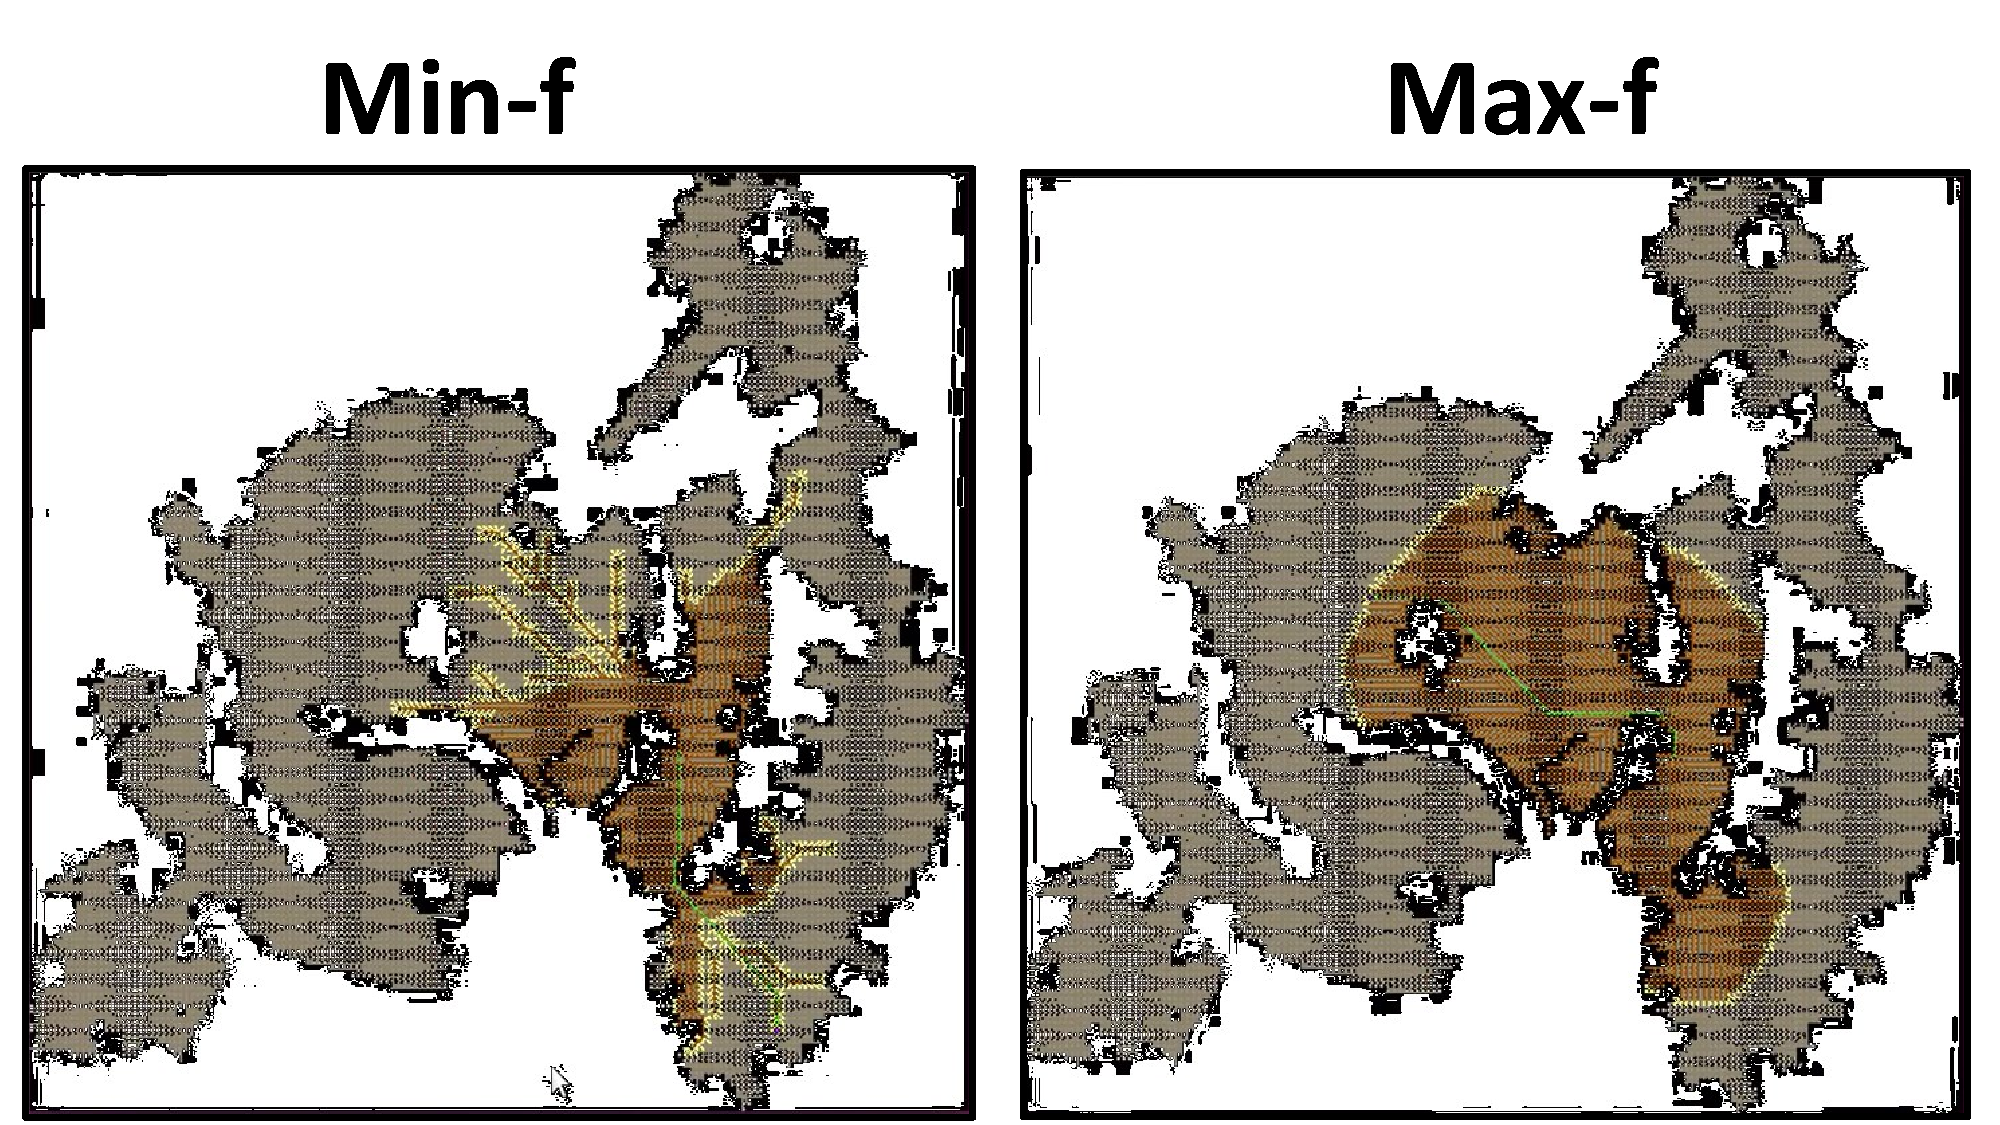
\includegraphics[width=\columnwidth]{min-vs-max}
  \caption{An example of running \kastarmin (left) and with \kastarmax (right).
  The yellow parts represent the states in \open, the brown parts represent the states in \closed.
  To see a running example of how \open changes throughout the search in this example see the videos in the following URLs \emph{http://tinyurl.com/ze29tb4} (for \kastarmax) and     \emph{http://tinyurl.com/zawrmtd} (for \kastarmin). [[AF: change the terms above the figure to be consistent with the text in the paper]]}
  %\textsc{in the following URLs \url{http://tinyurl.com/ze29tb4} (for \kastarmax) and     \url{http://tinyurl.com/zawrmtd} (for \kastarmin).}
  \label{fig:min-vs-max}
\end{figure}


An interesting observation is that \kastarmax is faster than Eager \kastarmin when the number of goals is large (see $k=64$ and $128$).
To explain this, consider the illustrations in Figure~\ref{fig:min-vs-max}.
They show an example of running \kastarmin (left) and \kastarmax (right) on the same \kgs instance.
The yellow points represent states in \open, the brown points represent states in \closed, the graph points are states that were not generated so far, and the white points and the black points are impassable obstacles.
As can be seen, the behavior of \kastarmin and \kastarmax are different: \kastarmin runs greedily towards prospective goals, showing clear trajectories protruding from the search frontier, while \kastarmax demonstrates a behavior that is more similar to uniform cost search.
This occurs because when a child is generated in \kastarmin, if it is closer to the closest goal than its parent then it will be expanded next, resulting in these protruding DFS-like trajectories towards the goal.
By contrast, in \kastarmax even if a state generates a child state that is closer to the closest goal, it still may not be expanded because it is further from some other goal.
This results in having \kastarmax behaving in a somewhat similar manner to UCS, and thus for large number of goals its \open will contain fewer states than \kastarmin.\footnote{Having fewer states in \open also impacts the costs $C_{gen}$ and $C_{r}$, since we implemented \open using a binary heap, and thus the runtime of reordering \open and inserting states into \open depends on the size of \open.
Indeed, the assumption that $C_{gen}$ and $C_r$ are constant throughout the search is only an abstraction of the true costs, which depends on the exact implementation. [[AF: footnote appeares two pages from the text. Maybe just put it in the main text}


%\roni{Probably there's a nicer way to explain this.} [[AF: Yes there is. We need to think]] This behavior results in \kastarmin having a weaker duplicate detection phase compared to \kastarmax, resulting in a bigger \open and thus more generated states. \roni{Can anyone explain why Lazy \kastar generates more states?} [[AF: Lazy should be identical to \kastarmin. Maybe they had different tie breaking?]]


%\begin{figure}
%   \includegraphics[width=0.45\columnwidth]{Capture-minf.PNG}
%   \includegraphics[width=0.45\columnwidth]{Capture-maxf.PNG}
%   \caption{XXx}
%   \label{fig:min-vs-max}
%\end{figure}


\subsubsection{The Impact of the Distance between Goals}

\begin{figure}
  \centering
  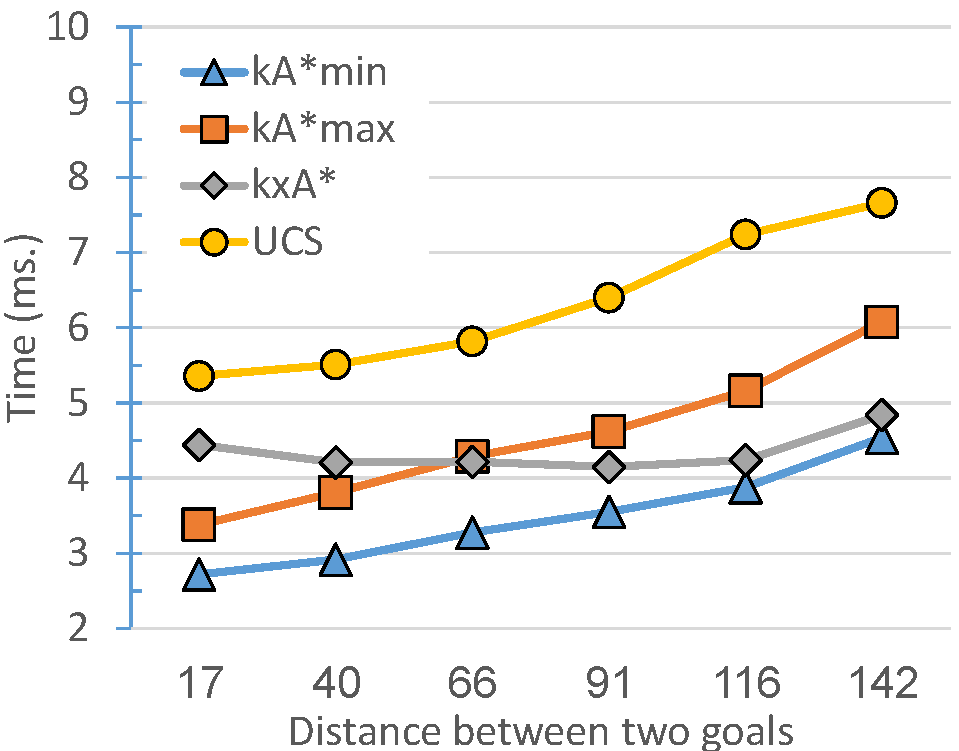
\includegraphics[width=0.5\columnwidth]{G0-G1-focused_cropped.pdf}
  \caption{This figure plots the runtime (in ms.) of the different \kgs algorithms as a function of the distance between the goals, for a \kgs problem with two goals ($k=2$).}
  \label{fig:2-goal}
\end{figure}

In the second type of experiments we performed, we focused on \kgs problems [[AF: instacnes??]] with two goals ($k=2$), and investigated the impact of the distance between these goals on the effectiveness of the evaluated algorithms.

%\roni{TODO: Fill in with Meir: how was the random walks performed, how was the binning, etc.}

The results are given in Figure~\ref{fig:2-goal}.
The $x$-axis is the distance between the goals, and the $y$-axis shows the average runtime in milliseconds of the different algorithms.
We compared Lazy \kastarmin, \kastarmax, \kxastar, and UCS.
We observe several trends.
First, for a 2-goal problem it is clear that uniform cost search is the worst option.
This is reasonable as UCS is only effective when the number of goals is large (since it does not use a heuristic).
%This is reasonable, as it does not use a heuristic to guide its search and the number of goals is small.
Second, observe that when the goals are close to each other, both \kastarmin and \kastarmax outperform \kxastar.
This matches our analysis (Section~\ref{sec:resource-analysis}), where if the goals are close to each other we expect that many states will be expanded by both independent \astar searches, which is  exactly the redundancy \kastar was designed to solve.
More formally, when the goals are close to each other, then the intersection of $Gen(\text{\astari{1}})$ and $Gen(\text{\astari{2}})$ will be large and so $|Gen(\text{\astari{1}})\cup Gen(\text{\astari{2}})|$ will be significantly smaller than $|Gen(\text{\astari{1}})|+|Gen(\text{\astari{2}})|$, providing an advantage to \kastarmin (see Table~\ref{tab:time-analysis}).
Following this explanation, we observe that as the goals chosen become distant from each other (going right on the $x$ axis of Figure~\ref{fig:2-goal}), we see that the advantage of \kastar over 2 \astar searches diminishes.  [[AF:maybe write  "2 X A*"]]
Indeed, the performance of \kastarmin and \kxastar converge when the goals are furthest from each other.
Lastly, we observe that \kastarmin dominates \kastarmax and in general all other approaches, always being better or on par with the other algorithms.

\subsubsection{The Impact of Using Stronger Heuristics}

\begin{figure}
  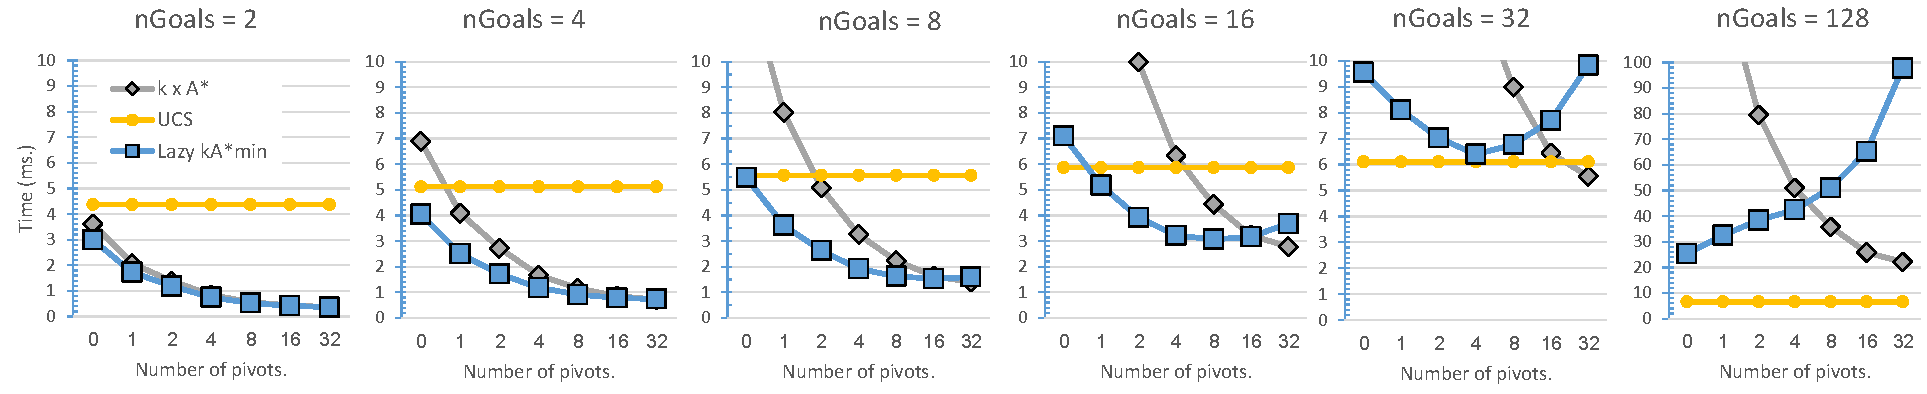
\includegraphics[width=\textwidth]{heuristic-power_cropped.pdf}
\caption{The runtime of Lazy \kastarmin, \kxastar, and UCS for different number of goals (the different plots) and difference number of pivots using in the heuristic computation.
With more pivots, the heuristic is more accurate but slower to compute.}
  \label{fig:dh-results}
\end{figure}

Next, we evaluated the impact of using a stronger, more accurate heuristic, on the performance of the proposed \kgs algorithms.
To this end, we used differential heuristics (DH)~\cite{goldberg2005computing,ng2002predicting,SturtevantFBSN2009} instead of Octile distance.
DH is a more sophisticated memory-based heuristic for grid pathfinding that works as follows.
A set of states (cells in the grid) are chosen  referred to as the \emph{pivots}.
Then, in a pre-processing step, we compute and store in memory a shortest path between every state and these pivot states.
When computing the heuristic for a state that is not part of these states, one can use the triangle inequality to obtain an admissible heuristic.
For more details, see~\cite{goldberg2005computing,ng2002predicting,SturtevantFBSN2009}.
Importantly, adding more pivots results in a more accurate heuristic, but one that takes longer time to compute.


Thus, DH is especially useful for our analysis, as it can be tuned to more accurate and more costly to compute.
The results of Lazy \kastarmin, \kxastar and UCS are given in Figure~\ref{fig:dh-results}.
The different plots show the results for 4, 8, 16, 32, 64, and 128 goals.
The $y$ axis shows the average runtime in milliseconds and the $x$ axis shows the number of pivots used for computing the heuristic.
As expected, the runtime of UCS is unaffected by the number of pivots, since it does not use a heuristic.
Also, if we fix the number of pivots and observe the impact of increasing the number of goals, the benefit of using heuristic search over plain UCS diminishes.
Eventually, when solving for 128 goals, UCS dominates both \kastarmin and \kxastar.
This follows the same trends observed for the Octile distance results given in Table~\ref{tab:pathfinding-runtime}, and the explanation we provided for these results hold here too.
%is the same as tehre. %solving for large number of goals eventually

%[[AF: in the figure please reword the "per Goal" to be consistent with the terminology in this paper. In other places too.]]

Next, consider the impact of adding pivots --- i.e., using a stronger but more costly heuristic.
For \kxastar, we observe that adding pivots always helps reducing runtime.
For \kastarmin, however, adding pivots improves runtime only for cases when the number of goals was not very large.
For example, when $k = 32$, using more than 4 pivots actually degrades the performance of \kastarmin.
These results conform with out theoretical analysis: adding pivots increases $C_h$, which is incurred more times in \kastarmin than in \kxastar (see Table~\ref{tab:time-analysis}).

[[AF: Roni, I am not sure why you are pessimistic. In most of the points of this figure, \kastarmin is the best. This is very encouraging because this is the middle ground with reasonable number of pivots and reasonable number of goals ]]

\subsection{Pancake Puzzle}

Next, we present the results for the pancake puzzle.
The heuristic used was the GAP heuristic~\cite{helmert2010landmark}, adjusted so that it is suitable for different goal states.
%\roni{Meir: what was the heuristic used? how were the states generated? how many instances?}
We experimented with 1, 2, 4, 8 and 16 goals ($k$).
For every $k$ we generated 100 random instances, where goal $g_1$ was the standard pancake goal state (where the pancakes are stacked by size) and the other goals are random permutations. %[[AF: so in fact, it is equivalent to the case where they are all random permutations]]\roni{Not sure why we should mention this?}

\begin{table}
  \centering
  \caption{Running time (in ms.) and number of generated states for solving \kgs with two goals in the Pancake puzzle domain using UCS and \kastarmax.}
  \label{tab:pancake-max-uniform}
  \begin{tabular}{lrrrr}
    \toprule
    \# Pancakes & \multicolumn{2}{c}{Runtime (ms.)} & \multicolumn{2}{c}{Generated} \\
    \cmidrule(lr){2-3} \cmidrule(l){4-5}
                & \kastarmax & Uniform & \kastarmax & Uniform \\
    \midrule
    6           &   0.34     &   0.46     &     994             &     2,287 \\
    7           &   2.57     &   4.06     &   8,617             &    21,059 \\
    8           &  22.95     &  40.25     &  74,745             &   188,946 \\
    9           & 410.81     & 717.64     & 787,481             & 1,973,420 \\
    \bottomrule
  \end{tabular}
\end{table}


The first result we report is that UCS and \kastarmax could not solve even small-sized problems even for $k=2$.
Average runtime and number of states generated for $k=2$ and pancakes of size up to 9 are given in Table~\ref{tab:pancake-max-uniform}.
These results are not surprising, because in exponential domains running a search without a heuristic is not practical, and \kastarmax can behave similar to UCS (as shown also in Figure~\ref{fig:min-vs-max}).

\subsubsection{The Impact of Varying the Number of Goals}
\newcommand{\tbf}[1]{\textbf{#1}}
\begin{table}
  \centering
  \caption{The average runtime and average number of states generated in the pancake experiments, for \kastar with \minf and for running $k$ independent \astar searches.
  Best results per $k$ are highlighted in bold.}
  \label{tab:pancake-minf-k-searches}
  \begin{tabular}{rrrrrrrrr}
   \toprule
  $k$ & \multicolumn{4}{c}{10 Pancakes} & \multicolumn{4}{c}{20 Pancakes} \\
   \cmidrule(r){2-5}\cmidrule(l){6-9}
      & \multicolumn{2}{c}{Runtime (ms.)} & \multicolumn{2}{c}{Generated} & \multicolumn{2}{c}{Runtime (ms.)} & \multicolumn{2}{c}{Generated} \\
   \cmidrule(r){2-3}\cmidrule(lr){4-5} \cmidrule(lr){6-7}\cmidrule(l){8-9}
      & \kastarmin & \kxastar & \kastarmin & \kxastar & \kastarmin & \kxastar & \kastarmin & \kxastar \\
   \midrule
1  & 0.09 & \tbf{0.08} &   \tbf{190} & \tbf{190} &  4.24 & \tbf{4.17} & \tbf{7,324} & \tbf{7,324} \\
2  & 0.20 & \tbf{0.16} &   \tbf{363} &     368  &   9.75 &  \tbf{7.81} & \tbf{13,794} &    13,828 \\
4  & 0.51 & \tbf{0.35} &   \tbf{755} &     788  &  21.74 & \tbf{13.73} &    25,154 & \tbf{24,982} \\
8  & 1.18 & \tbf{0.67} & \tbf{1,364} &   1,512  &  66.63 & \tbf{30.14} & \tbf{53,268} &    53,790 \\
16 & 3.24 & \tbf{1.35} & \tbf{2,645} &   3,058  & 206.03 & \tbf{59.51} & \tbf{103,674} &  105,863 \\
  \bottomrule
  \end{tabular}
\end{table}

\kastarmin and \kxastar were able to solve larger pancake puzzle instances.
Therefore, we were able to evaluate  the impact of varying the number of goals on their performance.
Table~\ref{tab:pancake-minf-k-searches} presents their results for the 10 and 20 pancakes puzzle and different number of goals.
As expected, \kastarmin usually generates fewer states.
Nonetheless, the difference, in terms of number of states generated, is very small in this domain.
Moreover, the runtime of \kastar is constantly larger than the runtime of \kxastar, and the difference between them grows when the number of goals increase.
This is because in exponential domains the intersection between the sets of states generated by each search is small compared to size of the last $f$ layer of each search which is quite large.

[[AF: this is not a negative result]]

%\roni{Meir and Ariel, I'm looking for a nicer explanation. Any thoughts?}\roni{I am not sure how the ``denied'' column help explain this. If we have many denied states doesn't it mean that the intersection was actually large? }[[AF: I added some text but I think it is OK]]


\begin{figure}
  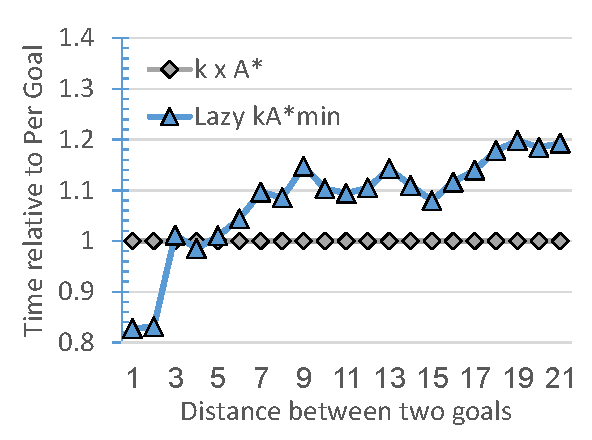
\includegraphics[width=\columnwidth]{pancake-goal-distance_cropped.pdf}
  \caption{10 pancake domain. Runtime as a function of the distance between the goals in \kgs with two goals.}
  \label{fig:2-goal-pancake}
\end{figure}

\subsubsection{The Impact of the Distance between Goals}

Next, we evaluated the impact of varying the distance between the goals, focusing on \kgs problems with two goals.
To do so, we generate 1,000 problem instances for this experiment by choosing the standard goal state (where all pancakes are ordered nicely) and performing a fixed number of random walks from it: 10 problem instances were generated by a single random step from the standard goal, the subsequent 10 problem instances were generated by two random steps from the standard goal, and so on.
Then, each instance was solved optimally to find the exact distance between the goals, and the results of instances with similar distance were bucketed together.

%To gain a deeper insight into the behavior of the various \kgs algorithm in this domain, we performed additional experiments.

Figure~\ref{fig:2-goal-pancake} plots the runtime of Lazy \kastarmin and \kxastar for these \kgs instances with different distances between them (depicted in the $x$-axis).
Here, we show the relative runtime of \kastarmin compared to \kxastar.
So values smaller than one correspond to cases where \kastarmin was faster than \kxastar and values larger than one correspond to cases where \kxastar was faster.

As we observed in the grid path finding domain, when the goals are very close, \kastarmin is better that \kxastar, as there is a large intersection between the states generated by the individual \astar searches.
However, we observe here that unlike the grid path finding domain, the advantage of \kastarmin quickly disappears, and for cases where the goals are more than 5 steps apart it is better to use \kxastar.
To explain this, note that the pancake puzzle is an exponential domain.
Therefore, even if the two goals are relatively close to each other, the search spaces corresponding to finding each of them can be them may have a relatively small overlap.
Consequently, \kastarmin will perform poorly compared to \kxastar.

% This supports our analysis, as in exponential domains a small distance between the goals can result in needing a very large number of unique states to expand per goal.

To conclude our experimental results, we observed the following trends:
\begin{enumerate}
  \item Eager \kastarmin usually outperforms \kastarmax, but not always.
  Lazy \kastarmin outperforms both.
  \item When the number of goals becomes very large, simply running UCS is the best option, as it does not spend time on heuristic computations.
  \item In the grid pathfinding domain, which is a polynomial domain, many states are generated by more than one search, and consequently \kastar is advantageous compared to \kxastar searches.
  \item In the pancake domain, which is an exponential domain, only relatively few states were generated by more than one search, and so running $k$ individual searches (\kxastar) is usually faster than running \kastar, unless the goals are very close to each other.
\end{enumerate}

[[AF: I eould reverse the last item. Say, that for small distances \kastar was better but for large distances  \kxastar was better]


\section{Related work}
\label{sec:related-work}

\kgs is similar to many previously studied problems.
As mentioned in the introduction, \kgs is different from TSP in that the task in TSP is to find a
shortest path that passes through a set of vertices, while in \kgs the task is to find $k$ shortest path, one to each vertex.
%In that sense it is similar to the minimal spanning tree (MST) problem, but we only require optimal path to a selected set of $k$ vertices and not to all vertices (as in MST).

\kgs is also different from a disjunction of $k$ goals, i.e., from the case where there are $k$ possible goals and the task is to find a lowest-cost path to [[AF: the closest]] one of them.
Unlike this case of a disjunction of $k$ goals, in \kgs we must find a shortest path to each of the goals, and not just to the closest one.
Other related problems are the problem of finding $k$ disjoint paths between a two vertices~\cite{suurballe.jw:disjoint} and the problem of finding the best $k$ paths between two vertices~\cite{pollack.m:letter,Eppstein1998}.
These are different problems from \kgs since in \kgs we have $k$ different goals.

Somewhat related is the work on \emph{multi-objective search}, where we have multiple objectives function that we wish to optimize~\cite{machuca2011analysis}.
For example, in a navigation application one may want to optimize for path length and also for ease of navigation.
An optimal solution to a multi-objective optimization problem is usually a solution that is Pareto optimal, and it is often the case that one would like the set of all Pareto-optimal solutions.
This is fundamentally different from \kgs, where we have a single optimization criteria --- we must have a lowest-cost path to each of the $k$ goals.

The \kgs problem is related to the problem addressed by incremental search algorithms such as Lifelong Planning \astar~\cite{koenig2004lifelong}, D$^*$-Lite~\cite{koenig2005fast}, and Path-Adaptive \astar~\cite{hernandez2015reusing}.
Incremental search algorithm are designed to solve a sequence of search problems, where the start and goal of these search problems are the same, but the underlying graph has changed.
The key idea in incremental search algorithms is to re-use information from previous searches to solve faster the current search problem.
The incremental search setting is different from \kgs: in incremental search we have one goal and the environment is dynamic, while in \kgs we have $k$ goals but assume the environment does not change.
Another related problem is the moving-target search problem~\cite{koenig2007speeding,IshidaK1995}.
A moving-target search problem is a search problems where the goal changes during the search.
This is different from \kgs where we have $k$ goals, and the goals do not change during the search.
Exploring how ideas from incremental search and moving-target search may be imported to help solve \kgs problems is left for future work, and we outline below some exciting directions. [[AF: Nice. But, maybe you want to say that before so as to better motivate taking on these problems which seem quite different than our problem]]


\section{Conclusion and Future Work}

In this work we studied the \kgs problem, and analyzed two fundamental approaches for solving it: $k$ single-goal searches (\kxastar) and a single search for $k$ goals (\kastar).
We analyzed the deficiencies of \kxastar and proposed several variants of \kastar: \kastarmax, Eager \kastarmin, Eager$^+$ \kastarmin, and Lazy \kastarmin.
Given an admissible heuristic, both Eager, Eager$^+$, and Lazy \kastarmin are sound and complete, and if the heuristic is consistent so is \kastarmax.
We then analyzed all the proposed algorithms theoretically, comparing their memory requirements and runtime.
This analysis provided guidelines for when to use which algorithm.
These guidelines were then tested in practice in two representative domains: one with a state space that is polynomially in the input and one with a state space that is exponential in the input. Empirically, we showed that Lazy \kastarmin dominates the other \kastar variants.
In addition, our results suggest that in polynomial domains it is usually the case that running \kastar is better than \kxastar, but in exponential domains \kxastar is usually better. [[AF: Usually? Maybe better market the cases where \kastar was better]]
Finally, if the number of goals is very large then running UCS is the best option.

This work is, to the best of our knowledge, the first study of using heuristic search techniques to solve \kgs.
There are several exciting directions for future work.
First, we only explored in this work how to avoid some of the redundant computations done when performing $k$ individual searches.
As mentioned briefly in Section~\ref{sec:kxastar}, a different way to benefit from searching for multiple goals is to learn valuable information about the underlying graph while searching for one goal, and use this information to improve the search for the other goals. % This can include, for example, using learning techniques to improve the quality of the heuristic.

%We give two possible directions for future work where such learning fromexperience can occur.
One way to learn such information so is use knowledge about the shortest path found so far to improve the quality of the available heuristics.
For example, in undirected graphs the difference between the heuristic for one goal and the heuristic between goals is an admissible heuristic by itself, which may be more accurate than the given heuristic $(h_1, \ldots h_k)$.
%[[AF: better explain what you mean. What is your new heuristic? Define it precisely.]]\roni{No, this is a future work section, not the body of the paper. Defining things precisely would be too formal for this part of the paper.}
This idea is inspired by path-finding memory-based heuristics such as Differential heuristics and others~\cite{sturtevant2007memory,SturtevantFBSN2009,goldenberg2011theCompressed}.


Another way to learn information about the search space is to compile \kgs to an incremental search problem.
A possible approach to do so is by adding an artificial vertex that is connected to all goals, and running the search from this goal to the start state.
Then, every iteration of the incremental search algorithm will change the weight of the edges from the artificial goal to the actual goal, setting the edge to exactly one goal with zero weight and all other edges as unpassable.
There are several challenges in implementing this compilation approach, such as how to choose the order of goals that will be solved, so as to optimize the amount of information learned between searches.
The benefit of such a compilation approach is that that it may enable using incremental search algorithm such as Path-Adaptive \astar~\cite{hernandez2015reusing} to solve the \kgs problem.
Also, we believe that a similar approach for solving \kgs can be done by compiling it to a moving target search problem.

[[AF: Why not mentioning bidirectional search?]]

% \begin{figure}[!htbp]
%   \centering
%   \includegraphics[width=1\hsize]{filename.eps}
%   \caption{caption} \label{fig:label}
% \end{figure}

\acks{Financial support for this research was in part provided by Israel Science Foundation (ISF) grant \#417/13. 
We also wish to thank the anonymous reviewers that reviewed a preliminary version of this work that was submitted to AI Comm. Their comments were invaluable. 
}


\appendix
\section*{Using Max as a Heuristic Aggregation Function}

[[TODO: PUT HERE ALL THE FMAX STUFF]]

\section*{Stuff}

in the following section a single search 

Specifically, 
to avoid expanding a node multiple times, we propose the different searches share \open and \closed 

we propose a \kgs algorithm in which the different searches share , we propose an information sharing 

%Both of these potential sources of improvements  over \kxastar are based on sharing information between the $k$ searches of \kxastar. To avoid expanding a node multiple times, we can share  \open and \closed between the searches. That is, , passing \open and \closed

More generally, we identify the following two potential sources for improvement over \kxastar when solving a \kgs instance. 
\begin{itemize}
\item \textbf{Avoiding expanding a node multiple times.}
  The same node can be expanded by multiple \acp{SPP}.
  For example, \kxastar generates the children of the start at least $k$ times.
  This introduces redundancy to the search process that may be avoided by sharing \open and \closed across searches. 
  
\item \textbf{Using updated low-cost paths to nodes.}
  The lowest-cost path to a node found so far in the search is stored in its $g$ value, and can get updated as the search progresses. Updating the $g$ value is commonly done within an individual search, but in the context of \kxastar{} one may also migrate updated $g$ values across searches.
  %[[AF: we note that]] 
  %Updating the $g$ value of a node may require updating the position of that node in \open and, if the heuristic is inconsistent, even expanding that node multiple times in the same search. 
\end{itemize}
%Both of these potential sources of improvements  over \kxastar are based on sharing information between the $k$ searches of \kxastar. To avoid expanding a node multiple times, we can share  \open and \closed between the searches. That is, , passing \open and \closed




When the first \astar search in \kxastar (i.e., \astari{1}) starts, its \open contain $s$ and its \closed is empty, as in any standard \astar.
Then, when \astari{1} finishes its search (with an optimal path to $t_1$), it passes \open and \closed to \astari{2}.
This includes the $g$ value of all the nodes generated by \astari{1}, and in some implementations also their $h$ values.\footnote{While it is possible not to store the $h$ value of a state and re-compute it every time the search needs the $f$ value of that state, standard implementation [[AF: standard? maybe time aware? BTW, you store the f value because open is sorted accordingly. And if you also know g then you know h too because f=g+h.]] of \astar usually stores the $h$ value of every generated state to save heuristic computation time.} 
If \closed contains $t_2$, we can halt since all the heuristics are consistent.[[AF: and $g(t_2)$ cannot decrease]]
Otherwise, we re-compute the $h$ and $f$ values stored for the states in \open using $h_2$ and $g+h_2$, respectively, and reorder these states to [[AF: in]] \open according to their up-to-date $f$ values.
This step is needed since the states were previously ordered in \open according to $f$ values computed with $h_1$.
Note that even if $t_2$ is in \open, we must still continue the search to verify that the optimal path to it has been found.
Then, the search continues as a regular \astar until $t_2$ is expanded.
This process continues, passing \open and \closed from \astari{2} to \astari{3} and so on, until all $k$ states have been expanded.


This information includes the set of nodes in \open and in \closed, and the information stored about them, namely their $g$ and $h$ values. 


\subsection{Sharing \open and \closed between Searches}

We first describe how to share \open and \closed between the $k$ \astar searches of \kxastar under the assumption that all the heuristics $h_1, \ldots h_k$ are consistent, and relax this assumption later. 

When the first \astar search in \kxastar (i.e., \astari{1}) starts, its \open contain $s$ and its \closed is empty, as in any standard \astar.
Then, when \astari{1} finishes its search (with an optimal path to $t_1$), it passes \open and \closed to \astari{2}.
This includes the $g$ value of all the nodes generated by \astari{1}, and in some implementations also their $h$ values.\footnote{While it is possible not to store the $h$ value of a state and re-compute it every time the search needs the $f$ value of that state, standard implementation [[AF: standard? maybe time aware? BTW, you store the f value because open is sorted accordingly. And if you also know g then you know h too because f=g+h.]] of \astar usually stores the $h$ value of every generated state to save heuristic computation time.} 
If \closed contains $t_2$, we can halt since all the heuristics are consistent.[[AF: and $g(t_2)$ cannot decrease]]
Otherwise, we re-compute the $h$ and $f$ values stored for the states in \open using $h_2$ and $g+h_2$, respectively, and reorder these states to [[AF: in]] \open according to their up-to-date $f$ values.
This step is needed since the states were previously ordered in \open according to $f$ values computed with $h_1$.
Note that even if $t_2$ is in \open, we must still continue the search to verify that the optimal path to it has been found.
Then, the search continues as a regular \astar until $t_2$ is expanded.
This process continues, passing \open and \closed from \astari{2} to \astari{3} and so on, until all $k$ states have been expanded.

Now, consider the case where the heuristics $h_1, \ldots h_k$ are admissible but not consistent.
In this case, when passing information from \astari{1} to \astari{2} it might be the case that $t_2$ has been expanded and is currently in \closed, but the optimal path to it has not been found yet.
[[ADD EXAMPLE FROM THE POWER POINT]][[AF: this is easy to understand. No need for an example in my opinion]]
Thus, if the heuristics are inconsistent then having $t_2$ in \closed supplied by \astari{1} is not a sufficient condition to ensure admissibility of the search (i.e., finding an optimal path to $t_2$).
In order to guarantee optimality, the $h$ and $f$ values of all the states in \open must be re-computed using $h_2$ and \open must be reordered according to these up-to-date $f$ values.
Then, the search can halt only when it is guaranteed that the $g$ value of $t_2$ is indeed optimal. This will be true either when $t_2$ is expanded or when the minimal $f$ value in \open is larger than or equal to the $g$ value of $t_2$.

[[Roni: maybe worthwhile to say all this more formally, maybe not. No, this is OK]]
[[Roni: maybe noting that we can't do lazy here? Lazy was not yet defnied]]

%Advantages 
Sharing \open and \closed in \kxastar can be beneficial because a state is only generated once, even if it is manipulated by more than one of the \astar searches, and the $g$ values of states get more accurate as we perform more searches and gain better knowledge of the search space.
More accurate $g$ values leads to more accurate $f$ values and to potentially expanding fewer states. [[Roni: is an example needed? AF: no need for an example. Relatively easy.]]

%Disadvantages 
However, sharing \open and \closed in \kxastar can also hurt performance.
%[[Roni: can this happen also with consistent heuristics, I believe so]]
\begin{itemize}
\item Memory consumption may increase since \open and \closed include all states generated or expanded by all the $k$ \astar searches.
%- For any $1<i\leq k$, \closed of search \astari{i} may contain states that are surplus for $\Pi_i$,  and \open may contain states that that \open for \astar run
\item Runtime may decrease [[AF: increase??]], since \open operations (insert, pop, reorder) now may work on a larger set of states
\item Runtime may decrease  [[AF: increase??]], since for $1<i\leq k$ we compute $h_i$ for every state in \open, including states from past searches.
Such states may not even be generated by \astari{i}, and thus computing $h_i$ for them is redundant.
[[Roni: I need some term like surplus states but for generated states. There is something like this I think in Meir's work?]]
\end{itemize}

\abda{Add an example for poor max-memory usage.}[[AF: I do not think that an example is needed. Everything here is easy]]

The last item is especially problematic, since heuristic computation can be very time consuming.
Thus, we propose the following \kxastar variant that shares some information between the searches but not all of it.

[[AF: you might want to give a name to this straightforward variant. Like "KxA-trivial-sharing"]


%We suggest between two types of information sharing: sharing only the $g$ values and sharing \open and \closed.


\subsection{Sharing Only $g$ Values between Searches}
In this \kxastar variant [[AF: give it a name??]] , we only share between the searches information on the best (lowest) $g$ value found for every generated states and its parent pointer.
That is, when \astari{2} starts, it is given a data structure, e.g., a hashtable, that contains the $g$ values stored by \astari{1} for every state it generated.
Then, when \astari{2} generates a node, it checks if there is a stored $g$ value for that node.
If so, then it sets this $g$ value to this node if it is better than its current $g$ value.
Otherwise, it updates the $g$ values stored.
This process continues, passing the $g$ values of all previously generated states from \astari{2} to \astari{3} and so on, until all $k$ states have been expanded.  [[AF: must say that you do not pass open and that the search starts from the start state]

Some details must be clarified in this \kxastar variant.
First, if the heuristics are consistent then every \astar search should also notify its subsequent \astar searches whether it expanded any of the remaining goals, notifying that an optimal path to is has been found, and there is no need to run a separate search to find it. [[AF: no need to notify the new search. You only start these searches for nodes that their optimal path was not yet found]

Second, every \astar search starts with \open containing only $s$ and an empty \closed.
Then, when a state is generated it is inserted to \open even if it has a stored $g$ value that is smaller than the one given to it by its current parent (the state that generated it).
This is because \open is not shared and needs to be reconstructed.
To see this, consider the children of the start state.
They will have a stored $g$ value immediately after the first \astar search, but we would like to insert them to \open anyhow to continue the new search.  [[AF: this must be said above in the technical description, I think]]

Comparing this \kxastar variant with the former [[AF: why not call them names. For example, "f-sharing k x A*" (fKxA*) vs. g-sharing gKxA* vs. baseline or basic KxA*. Or at least call them V1, V2, V3 etc.]], it shares the advantage that up-to-date $g$ values are used but the same state can be generated in more than one search.
Memory consumption is similar, as the $g$ values data structure holds the $g$ value for every state generated in all searches, however, \open and \closed are much smaller in the searches, and the heuristic is computed only to states that \astar would have generated. [[AF: also, no need to reorder open every time a new search starts]]

Thus, we cannot say that one \kxastar variant dominates the other in all domains. [[AF: no need for formal analysis but maybe an experimental comparison is needed. Also, maybe a table comparing the main differences should be given, like a column for sharing g ]]

[[TODO: SOME FORMAL ANALYSIS??]]







\vskip 0.2in
\bibliography{library}
\bibliographystyle{theapa}

\end{document}